%# -*- coding: utf-8-unix -*-
%%==================================================
%% thesis.tex
%%==================================================

% 双面打印
% \documentclass[doctor, openright, twoside]{sjtuthesis}
\documentclass[bachelor, openany, oneside, submit]{sjtuthesis}
% \documentclass[master, review]{sjtuthesis}
% \documentclass[%
%   bachelor|master|doctor|coursepaper, % 必选项,分别是学士,硕士,博士学位论文以及课程论文
%   fontset=fandol|windows|mac|ubuntu|adobe|founder, % 字体选项
%   oneside|twoside,        % 单面打印,双面打印(奇偶页交换页边距,默认)
%   openany|openright,      % 可以在奇数或者偶数页开新章|只在奇数页开新章(默认)
%   english,                % 启用英文模版
%   review,     % 盲审论文,隐去作者姓名、学号、导师姓名、致谢、发表论文和参与的项目
%   submit      % 定稿提交的论文,插入签名扫描版的原创性声明、授权声明
% ]

% 逐个导入参考文献数据库
\addbibresource{bib/thesis.bib}
% \addbibresource{bib/chap2.bib}

\newcommand{\sys}{Doraemon}
\newcommand{\li}{学习索引结构}
\newcommand{\cdf}{累积分布函数}
\newcommand{\rmi}{递归模型索引}
\newcommand{\lr}{线性模型}
\newcommand{\nn}{神经网络}

%# -*- coding: utf-8-unix -*-
% !TEX program = xelatex
% !TEX root = ../thesis.tex
% !TEX encoding = UTF-8 Unicode
%TC:ignore
\title{针对动态场景的{\li}的研究}
\author{唐楚哲}
% \author{某\quad{}某}
\advisor{王肇国副教授}
% \coadvisor{某某教授}
\defenddate{2019年XXX月XXX日}
% \coursename{某某课程}
\school{上海交通大学}
\institute{电子信息与电气工程学院}
\studentnumber{515030910448}
\cnacademicdegree{工学学士}
\major{软件工程}
\keywords{机器学习, 索引结构, {\li}, 动态场景}

\englishtitle{Learned Indexes for Dynamic Workloads}
\englishauthor{\textsc{Chuzhe Tang}}
\englishadvisor{Prof. \textsc{Zhaoguo Wang}}
% \englishcoadvisor{Prof. \textsc{Uom Uom}}
\englishschool{Shanghai Jiao Tong University}
\englishinstitute{\textsc{Depart of XXX, School of XXX} \\
  \textsc{Shanghai Jiao Tong University} \\
  \textsc{Shanghai, P.R.China}}
\englishinstitutemaster{Depart of XXX, \\ School of XXX}
\englishmajor{Software Engineering}
\englishdate{XXX XXX, 2019}
\enacademicdegree{Bachelor of Engineering}
\englishstudentid{515030910448}
\englishkeywords{Machine Learning, Index Structures, Learned Index Structures, Dynamic Workloads}
%TC:endignore
  % NOTE: the enclosed commands must be executed in preamble

\begin{document}

% 无编号内容:中英文论文封面、授权页
\maketitle
\makeatletter

\ifsjtu@coursepaper
\else
  \ifsjtu@submit\relax
    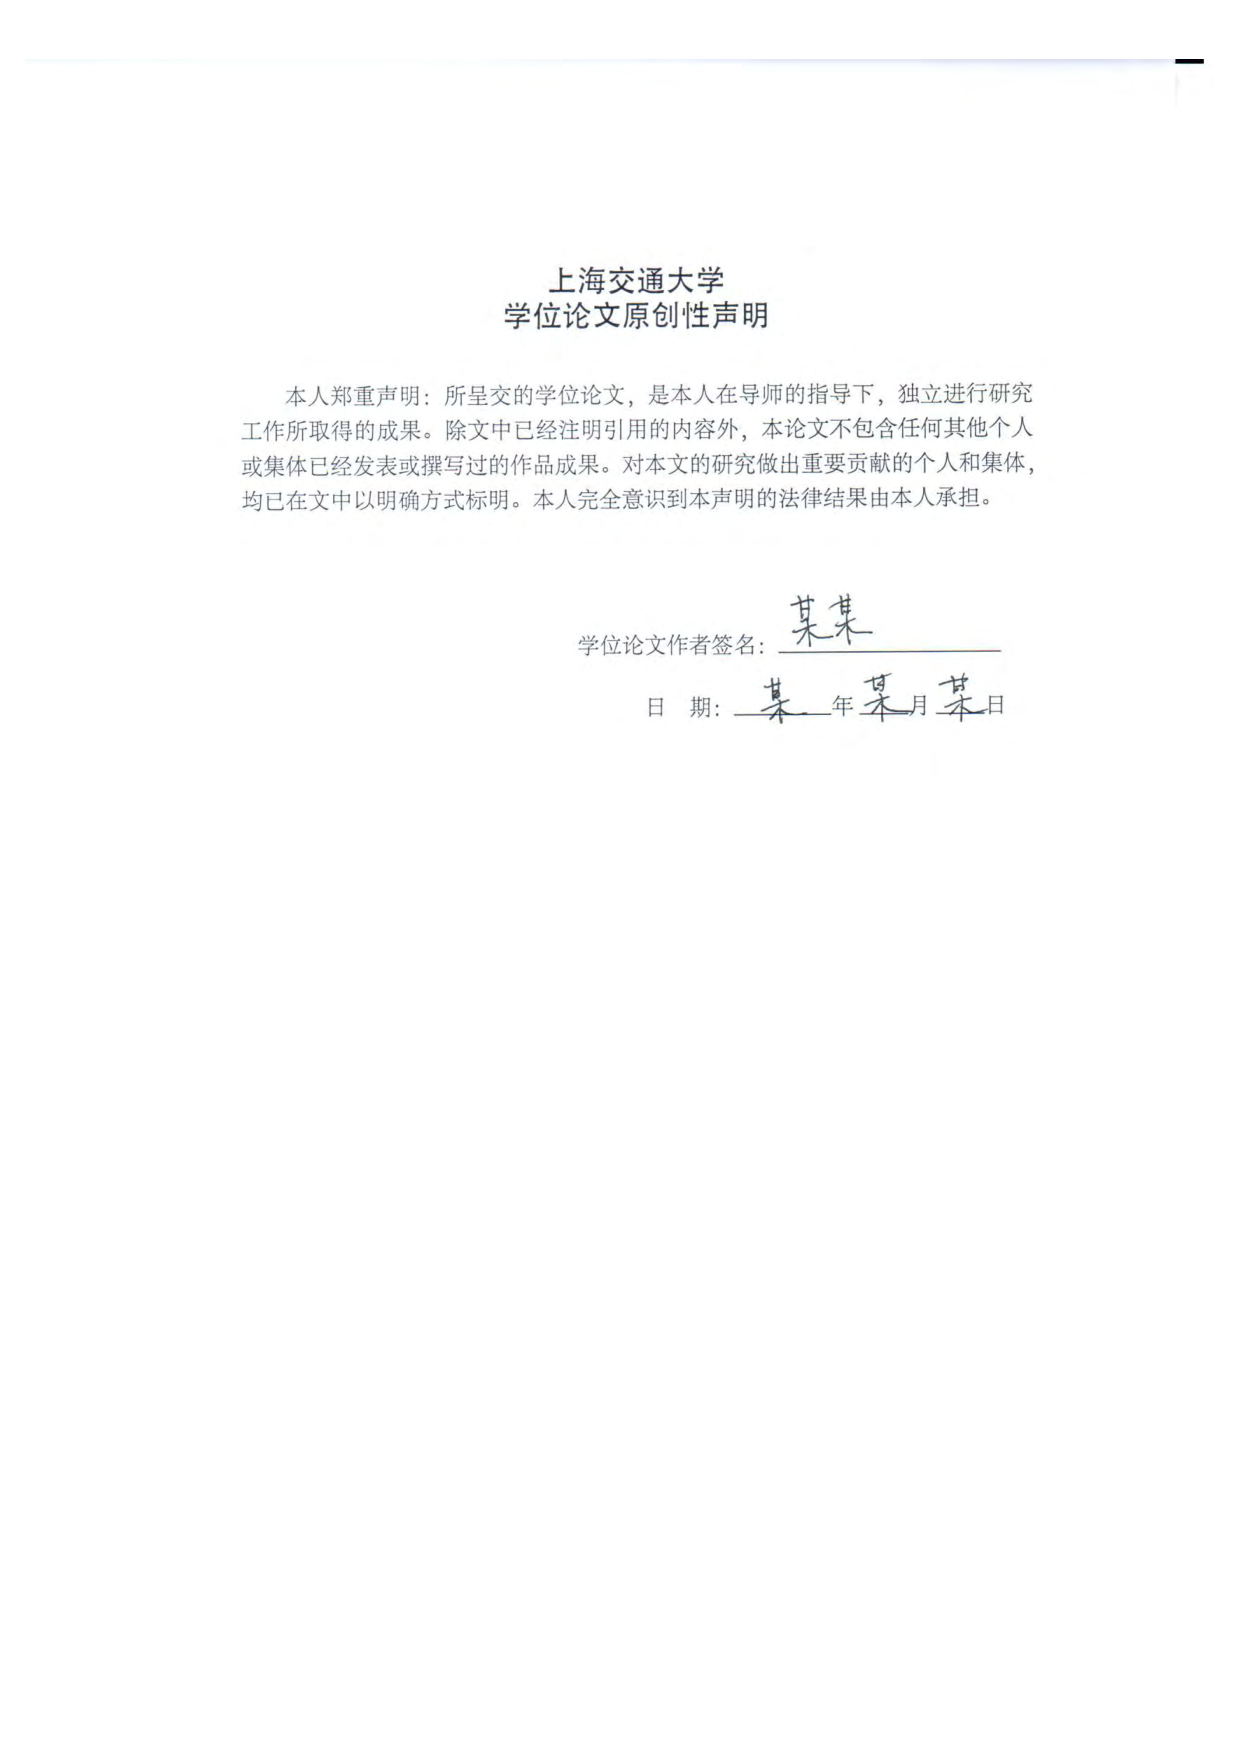
\includepdf{pdf/original.pdf}
    \cleardoublepage
    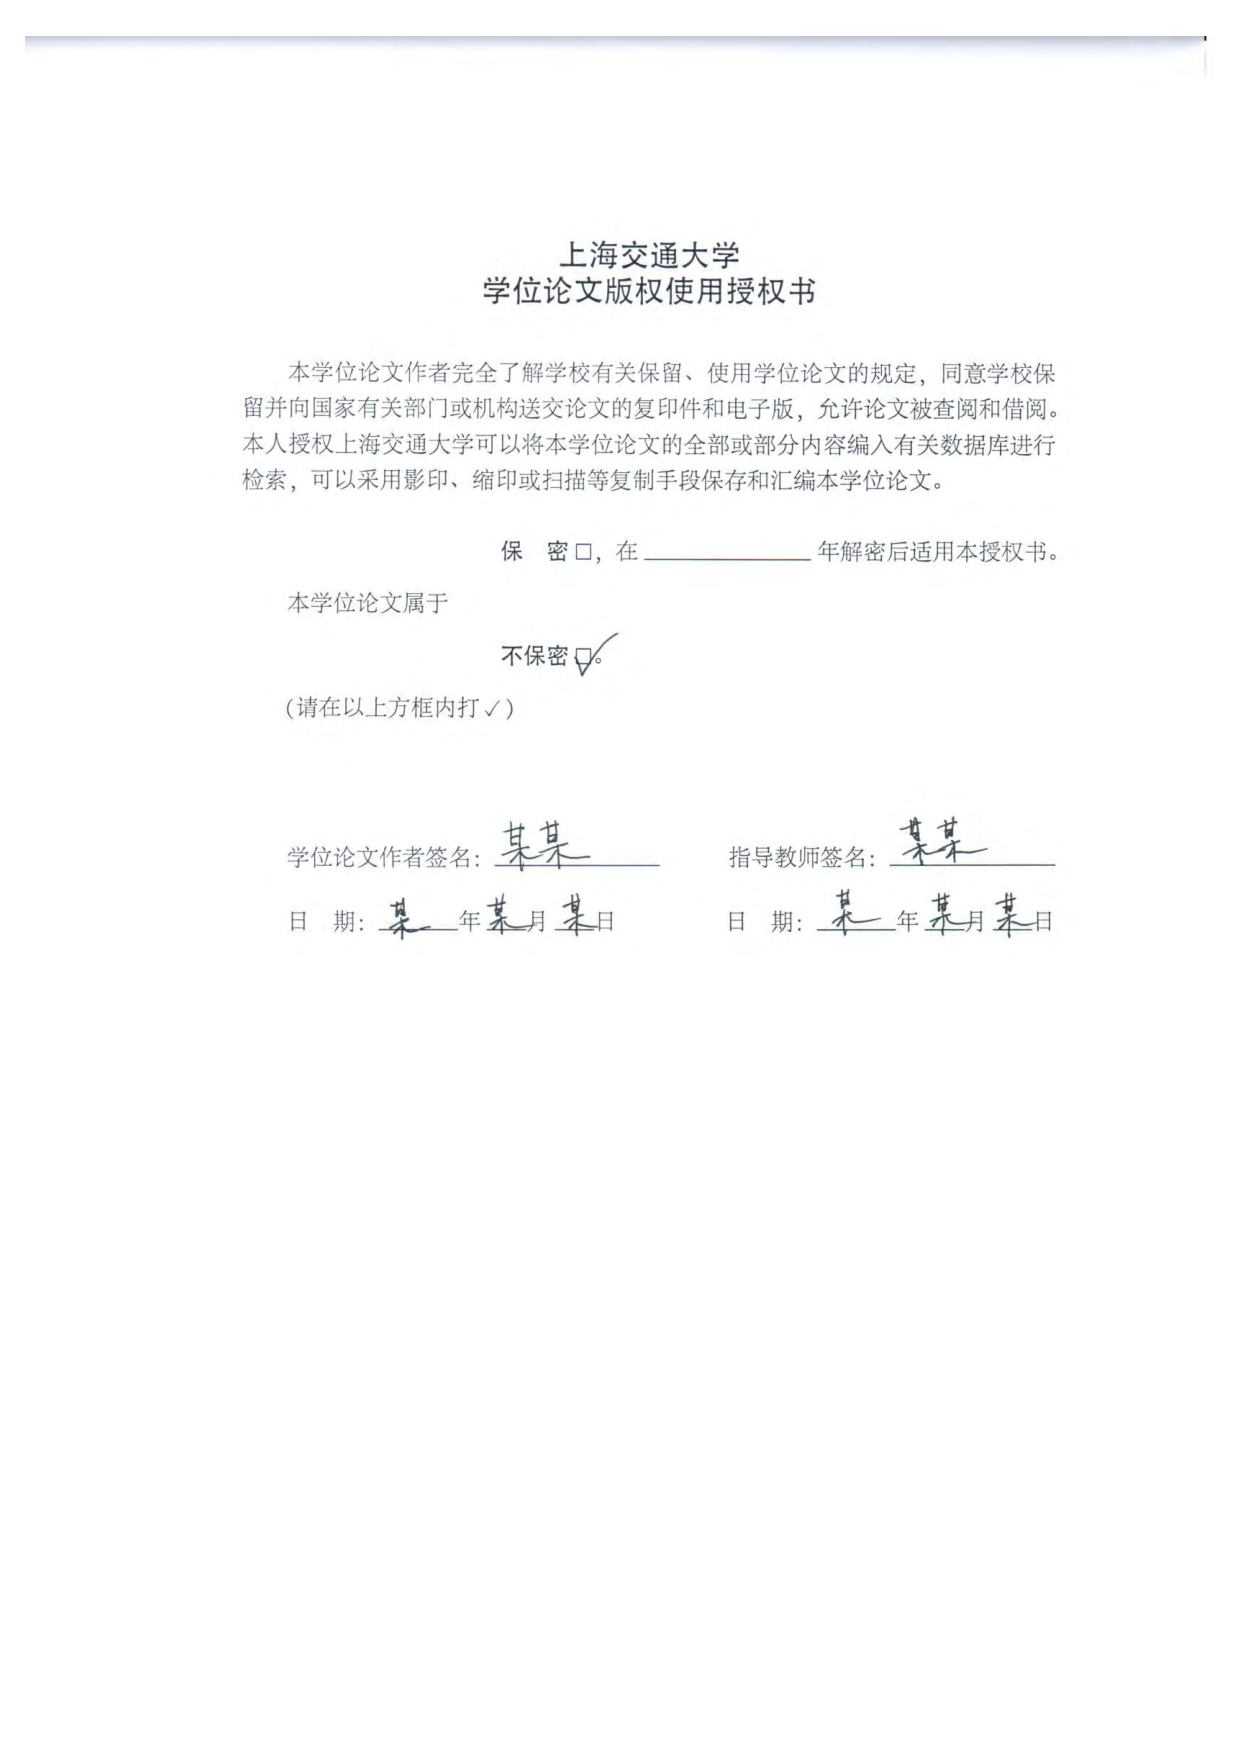
\includepdf{pdf/authorization.pdf}
    \cleardoublepage
  \else
    \ifsjtu@review\relax
    % exclude the original claim and authorization
    \else
      \makeDeclareOriginal
      \makeDeclareAuthorization
    \fi
  \fi
  \frontmatter % 使用罗马数字对前言编号

  % 摘要
  %# -*- coding: utf-8-unix -*-
% !TEX program = xelatex
% !TEX root = ../thesis.tex
% !TEX encoding = UTF-8 Unicode
%%==================================================
%% abstract.tex for SJTU Master Thesis
%%==================================================

\begin{abstract}

XXX

\end{abstract}

\begin{englishabstract}

XXX

\end{englishabstract}



  % 目录、插图目录、表格目录
  \tableofcontents
  \listoffigures
  \addcontentsline{toc}{chapter}{\listfigurename}     % 将插图目录加入全文目录
  \listoftables
  \addcontentsline{toc}{chapter}{\listtablename}      % 将表格目录加入全文目录
  \listofalgorithms
  \addcontentsline{toc}{chapter}{\listalgorithmname}  % 将算法目录加入全文目录

  %# -*- coding: utf-8-unix -*-
% !TEX program = xelatex
% !TEX root = ../thesis.tex
% !TEX encoding = UTF-8 Unicode
%TC:ignore
\begin{nomenclaturename}
\label{chap:symb}

\begin{longtable}{rl}
$\epsilon$     & XXX \\
%  $\mu$ 		& 磁导率 \\
%  $\epsilon$     & 介电常数 \\
%  $\mu$ 		& 磁导率 \\
%  $\epsilon$     & 介电常数 \\
%  $\mu$ 		& 磁导率 \\
%  $\epsilon$ 	& 介电常数 \\
%  $\mu$ 		& 磁导率 \\
%  $\epsilon$     & 介电常数 \\
%  $\mu$ 		& 磁导率 \\
%  $\epsilon$     & 介电常数 \\
%  $\mu$ 		& 磁导率 \\
%  $\epsilon$     & 介电常数 \\
%  $\mu$ 		& 磁导率 \\
%  $\epsilon$ 	& 介电常数 \\
%  $\mu$ 		& 磁导率 \\
%  $\epsilon$     & 介电常数 \\
%  $\mu$ 		& 磁导率 \\
%  $\epsilon$     & 介电常数 \\
%  $\mu$ 		& 磁导率 \\
%  $\epsilon$     & 介电常数 \\
%  $\mu$ 		& 磁导率 \\
%  $\epsilon$ 	& 介电常数 \\
%  $\mu$ 		& 磁导率 \\
%  $\epsilon$     & 介电常数 \\
%  $\mu$ 		& 磁导率 \\
%  $\epsilon$     & 介电常数 \\
%  $\mu$ 		& 磁导率 \\
%  $\epsilon$     & 介电常数 \\
%  $\mu$ 		& 磁导率 \\
%  $\epsilon$ 	& 介电常数 \\
%  $\mu$ 		& 磁导率 \\
%  $\epsilon$     & 介电常数 \\
%  $\mu$ 		& 磁导率 \\
%  $\epsilon$     & 介电常数 \\
%  $\mu$ 		& 磁导率 \\
%  $\epsilon$     & 介电常数 \\
%  $\mu$ 		& 磁导率 \\
%  $\epsilon$ 	& 介电常数 \\
%  $\mu$ 		& 磁导率 \\
%  $\epsilon$     & 介电常数 \\
%  $\mu$ 		& 磁导率 \\
%  $\epsilon$     & 介电常数 \\
%  $\mu$ 		& 磁导率 \\
%  $\epsilon$     & 介电常数 \\
%  $\mu$ 		& 磁导率 \\
%  $\epsilon$ 	& 介电常数 \\
%  $\mu$ 		& 磁导率 \\
%  $\epsilon$     & 介电常数 \\
%  $\mu$ 		& 磁导率 \\
%  $\epsilon$     & 介电常数 \\
%  $\mu$ 		& 磁导率 \\
%  $\epsilon$     & 介电常数 \\
%  $\mu$ 		& 磁导率 \\
\end{longtable}

\end{nomenclaturename}
%TC:endignore
 % 主要符号、缩略词对照表
\fi

\makeatother
\mainmatter % 使用阿拉伯数字对正文编号

% 正文内容
%# -*- coding: utf-8-unix -*-
% !TEX program = xelatex
% !TEX root = ../thesis.tex
% !TEX encoding = UTF-8 Unicode
%%==================================================
%% chapter01.tex for SJTU Master Thesis
%%==================================================

%\bibliographystyle{sjtu2}%[此处用于每章都生产参考文献]
\chapter{概述}
\label{chap:intro}

\section{研究背景}

作为一类重要的数据结构,索引在各种系统中发挥着重要的作用,其中包括操作系统(Operating System)、
数据库系统(Database)与文件系统(File System)等。
例如数据库系统中大量使用一级索引(Primary Index)和二级索引(Secondary Index)提高点查(Point Lookup)、
连接(Join)等操作的性能;文件系统常用基于inode的索引结构完成文件查找等操作。
传统的索引结构,包括B树(B-tree)、前缀数(Trie)与哈希表(Hash Table)在过去的几〸年内被广泛研究,
针对不同的应用场景,如读多写少、写多读少、大量小文件写操作等,各式各样的变种索引结构相继被提出[]。

2018年,谷歌提出基于机器学习的索引结构\cite{kraska2018case},将索引视为从键(Key)到数据位置的函数映射,通过多层级模型结构,
使用包括神经网络在内的多种机器学习模型拟合这一函数关系。
论文提出了三类学习索引:有序索引(Sorted Index)、无序索引(Unsorted Index)和存在索引(Existence Index),
其中有序索引与无序索引使用相同的模型设计,递归模型索引(Recursive Model Index,RMI)。
本文主要讨论使用递归模型索引的{\li}。
相比于传统索引结构,{\li}不能提供精确定位,相反{\li}为给定搜索键提供包含误差的预测位置和搜索范围。
对于存在的键,{\li}保证数据真实位置在给定的搜索范围内。
作为一种新型索引结构,{\li}去除了传统树状索引结构中存在的大量中间节点(Inner Node),不仅减少了查询的执行时间,
还降低了索引结构的空间消耗。

然而,原论文\cite{kraska2018case}对{\li}的测试与分析较为初步,甚至被一些研究人员认为会具有误导性\cite{throwalgo}。
他们假设工作场景是只读的,即被索引的数据是固定不变,{\li}不需要处理更新操作,并假设访问是均匀分布的,
即所有数据被访问的概率是相同的。
另一方面,在真实情景下,伴随着写操作的执行,索引数据是频繁变化的\cite{tpcc}。
同时,真实情景下数据访问是具有偏向性(Skewed)的\cite{zhang2016reducing, debrabant2013anti, eldawy2014trekking, levandoski2013identifying},
即数据存在冷热之分,大量数据访问发生在少量的热点数据上。
这些广泛存在于真实应用里的动态场景为{\li}的应用带来了许多挑战与机遇。

本文希望进一步探索分析{\li}在动态场景下所面临的挑战,并针对性地提出解决方案,拓宽{\li}的应用范围。

\section{研究现状}

本节将围绕{\li}与动态场景下的索引进行介绍。

\subsection{{\li}相关研究}

Michael\cite{NIPS2018_7328}对提出的存在索引\cite{kraska2018case},学习布隆过滤器(Learned Bloom Filter),进行数学建模与分析,
讨论了它相对于传统布隆过滤器不一样的性能保证,并分析了学习布隆过滤器对数据分布的要求。
基于数学分析,Michael通过在学习布隆过滤器前额外增加一层传统布隆过滤器,
提出三明治学习布隆过滤器(Sandwiched Learned Bloom filter)有效提高了学习布隆过滤器的工作性能。

Tim等人提面向分析处理的数据库SageDB\cite{kraska2019sagedb}。
SageDB提出通过机器学习对数据分布、工作场景与硬件环境进行建模,获得最优的数据结构、访问方式与查询执行计划。
具体的,SageDB广泛使用{\li}对一维与高维键进行索引。
对于高维键,SageDB提出使用映射的方式,将键从高维空间映射到一维空间中,从而使用原有的{\li}进行索引。
同时,SageDB拓展了{\li}的应用场景,讨论了磁盘数据与数据压缩等方面的可能性。

\subsection{动态场景下的索引结构}

相比于{\li},通用的传统索引结构通常不会对索引使用场景作过强的假设,
它们往往能够在不同的场景下都有类似的性能表现。
尽管如此,针对特定的动态场景,研究人员依旧通过设计出具体的索引结构变体,来提高在此场景下的索引性能。

Huanchen等人提出混合索引\cite{zhang2016reducing}(Hybrid Index),针对具有访问偏向性的动态场景进行优化。
混合索引通过冷热数据分离的方法,使用空间使用较少的、更新较灵活的热存储(Hot Store)来处理写操作,
用较为紧凑且只读的冷存储(Cold Store)来处理写操作,用较为紧凑且只读的冷存储(Cold Store)来存储大量的索引条目。
因为动态场景下的访问偏向性,热存储可以高效利用内存资源,并且减少索引延时,从而提供高吞吐量。

John等人提出分型树\cite{esmet2012tokufs}(Fractal Tree),针对写频繁且单次写数据量较少的动态场景进行优化。
分型树为每个节点配备了一定比例的缓存空间,所有的写操作都会先缓存在根结点里,
当节点缓存用尽后再被批量传播到各自对应的子节点中。
通过这种方法,对于频繁的小数据量写操作的动态场景,分型树将写操作带来的索引结构更新操作合并在一起,
减少索引结构更新操作对性能的影响。
同时,对于存在访问偏向性的动态场景,分型树的节点缓存能够很好地在索引树的较高节点位置处理热点数据的更新,
避免了数据的重复写入。

\section{主要研究内容}

本文首先介绍传统索引结构、机器学习与{\li}。
然后,结合测试与分析,本文探究在动态场景下,{\li}所面临的挑战以及挑战背后的原因。
具体的,我们探究动态变化的索引数据对{\li}性能的影响以及访问偏向性对{\li}性能的影响。
动态场景带来的挑战源自于两个方面,一是{\li}的性能依赖于架构选择与数据分布,并且难以通过数学表达式进行预测;
二是{\li}假设访问模式为均匀访问,从而在模型设计与训练的过程中缺乏对访问模式信息的有效利用。
针对以上原因,本文提出使用模型缓存(Model Cache)和数据拉伸(Data Stretching)的方法,
构建针对动态场景的学习索引系统,{\sys},来有效应对动态场景下{\li}面临的挑战,
同时保留{\li}的优秀特性,从而拓宽{\li}的应用范围。

总体来说,本文的贡献如下:
\begin{itemize}
  \item 探究并分析了{\li}在动态场景下面临的挑战;
  \item 提出了{\sys},一个针对动态场景的学习索引系统;
  \item 通过实验验证了{\sys}的有效性。
\end{itemize}

\section{论文组织结构}

本论文各章节的组织结构如下:

第一章阐述了本文的研究背景,对{\li}的相关研究以及动态场景下的索引结构进行了介绍,阐明了本文的研究内容以及文章的组织结构。

第二章对传统索引结构、机器学习以及{\li}相关背景知识进行介绍。

第三章介绍了在动态场景下{\li}面临的两大挑战:1)动态数据分布带来的挑战与2)动态访问模式带来的挑战,并详细分析了挑战背后的原因,
为{\sys}提供了分析支撑。

第四章提出了针对动态场景的学习索引系统,{\sys},并通过实验验证了本系统的有效性。

第五章总结全文,对本文的研究中的不足与局限之处进行了阐述,并针对性的提出了未来工作的展望。

%\bibliographystyle{sjtu2}%[此处用于每章都生产参考文献]
\chapter{相关技术背景}
\label{chap:back}

\section{传统索引结构}

索引是一类用于提高数据查询效率的数据结构。
传统索引结构按照数据结构可以分为基于树结构的索引与基于哈希函数的索引,根据功能可以分为范围查询索引、点查询索引和存在索引。
{\li}受传统索引结构启发与影响,了解传统索引结构有助于更好理解{\li}与本文的研究内容。

\subsection{B树及其变种}

B树及其变种索引结构是最常被使用的索引结构之一\cite{graefe2001b}。
B树是一种平衡的固定扇出(fanout)的树状结构,对于指定扇出值$B$,
B树保证除了根节点(root node)外所有节点包含的数据量大于$B/2$并小于$B$,
从而保证B树的树高$H=O(log_B(n))$,其中$n$为数据量大小。
平衡二分搜索树(balanced binary search tree)可以看作是一种扇出值为$2$的B树特例。
为保证节点数据量要求,当某节点数据量大于$B$时,该节点将会分裂为两个,
当某节点数据小于$B/2$时,该节点将与邻居节点进行合并。
B树树高为$O(log_B(n))$的特性使其插入(insert)、删除(delete)、
修改(update)与查找(lookup)均能在对数时间内完成,在大数据量下具有良好的性能表现。
B树及其变种索引结构因此被广泛地使用在数据库、文件系统与操作系统中。

% 在计算机科学中,B树(英语:B-tree)是一种自平衡的树,能够保持数据有序。
% 这种数据结构能够让查找数据、顺序访问、插入数据及删除的动作,都在对数时间内完成。
% B树,概括来说是一个一般化的二叉查找树(binary search tree)一个节点可以拥有最少2个子节点。
% 与自平衡二叉查找树不同,B树适用于读写相对大的数据块的存储系统,例如磁盘。
% B树减少定位记录时所经历的中间过程,从而加快存取速度。
% B树这种数据结构可以用来描述外部存储。
% 这种数据结构常被应用在数据库和文件系统的实现上。

分形树[](Fractal Tree)和B$^\epsilon$树[](B$^\epsilon$-tree)是B树的一种变种,它们与B树类似,
将数据排序并通过固定大小的节点进行索引,从而提供对数时间的性能。然而它们每一个节点包含一个缓存(buffer),
允许将插入、删除等修改操作临时保存在中间节点。
通过使用缓存,这些修改只会在积累了一定数量后,才会被写入下一级节点,从而避免了B树在索引磁盘数据时,
任何大小的写操作都会导致一次费时的磁盘读写操作。
然而,这种将修改进行缓存并批量传播的方式同时引入了写放大(write amplification)问题,
即对实际发生在系统里的写操作数据量,包括缓存的修改与传播,远大于用户真实写入的数据量。
尽管如此,分形树被使用在商业数据库TokuDB[]中,同时也在一些文件系统学术原型中[]被使用。

% In computer science, a fractal tree index is a tree data structure that keeps data sorted and allows searches and sequential access in the same time as a B-tree but with insertions and deletions that are asymptotically faster than a B-tree.
%  Like a B-tree, a fractal tree index is a generalization of a binary search tree in that a node can have more than two children.
%  Furthermore, unlike a B-tree, a fractal tree index has buffers at each node, which allow insertions, deletions and other changes to be stored in intermediate locations.
%  The goal of the buffers is to schedule disk writes so that each write performs a large amount of useful work, thereby avoiding the worst-case performance of B-trees, in which each disk write may change a small amount of data on disk.
%  Like a B-tree, fractal tree indexes are optimized for systems that read and write large blocks of data.
%  The fractal tree index has been commercialized in databases by Tokutek.
%  Originally, it was implemented as a cache-oblivious lookahead array,[1] but the current implementation is an extension of the Bε tree.
% [2] The Bε is related to the Buffered Repository Tree.
% [3] The Buffered Repository Tree has degree 2, whereas the Bε tree has degree Bε.
%  The fractal tree index has also been used in a prototype filesystem.
% [4][5] An open source implementation of the fractal tree index is available,[6] which demonstrates the implementation details outlined below.

% uses a fraction of node storage to serve as an
% update buffer \cite{esmet2012tokufs, bender2015and}.
% The updates will be flush to children's buffer when current node's buffer is full and applied until they
% reach the leaf.
% This optimization aims to avoid frequent small writes to disk.
% However, propagating updates also introduce write amplification problem.

Masstree[]是一种结合字典树(trie)和B树的索引结构,它将键分割为许多长度为8字节(Byte)的段(segment)并用字典树进行索引。
因为每一个段的长度较长,一个段可以有大量不同的可能值($2^32$,即$4294967296$),
因此每个字典树节点需要从大量的段值中快速查找出下一字典树节点的位置。
为解决单个字典树节点的查找性能问题,Masstree为每个字典树节点配备一个独立的B树。
当键的长度小于等于8字节时,Masstree等价于B树。
除此之外,Masstree是一个支持并发访问(concurrent access)的数据结构,它允许同时被多个线程(thread)发起读写操作。
在其内部实现中,Masstree使用乐观并发控制(optimistic concurrency control,OCC)保证对数据内容的读写原子性,
并使用细粒度锁机制(fine-grained locking)保证对元数据,包括内部节点,在更新操作下的一致性。

% \masst \cite{mao2012cache} partitions key into 8-byte segments and index them with a trie structure.
% Within each trie node, a concurrent \bt is used to index the segments.
% Similar to \sys, \masst uses optimistic concurrency control to ensure read/write atomicity and uses
% fine-grained locks to protect nodes during split and merge.

FITing-Tree[]是一个利用线性函数(piece-wise linear function)对B树操作时延(latency)与内存使用(memory consumption)进行优化的索引结构。
它通过使用线性函数拟合B树叶子节点(leaf node)中的数据分布,即键与位置的函数映射,达到节省内存空间的效果。
与B树不同之处在于,FITing-Tree并未限制叶子节点所包含的数据量,而是限制线性函数拟合结果的误差值(error)。
因为线性函数能够在给定的误差值范围内索引更多的数据,因此FITing-Tree的叶子节点远大于B树,从而降低中间节点的耗时,进而降低索引操作的时延。
相比于传统的节点结构,线性函数所需要的内存空间十分有限,从而节省大量的内存空间。
通过控制误差值,用户可以通过FITing-Tree的成本模型(cost model)预估其查询时延与内存使用情况,从而达到期望的性能表现。
然而,更新操作会使原有线性函数的误差值发生变化,违反用户指定的误差值,从而要求频繁对线性函数进行更新,造成索引性能下降。
为解决这一问题,FITing-Tree使用叶子结点内部缓存的方法,牺牲部分索引性能来降低对线性函数的更新频率。

% In this paper, we present a novel data-aware index structure called FITing-Tree which approximates an index using piece-wise linear functions with a bounded error specified at construction time.
% This error knob provides a tunable parameter that allows a DBA to FIT an index to a dataset and workload by being able to balance lookup performance and space consumption.
% To navigate this tradeoff, we provide a cost model that helps determine an appropriate error parameter given either (1) a lookup latency requirement (e.g., 500ns) or (2) a storage budget (e.g., 100MB).
% Using a variety of real-world datasets, we show that our index is able to provide performance that is comparable to full index structures while reducing the storage footprint by orders of magnitude.

Wormhole[]是一种结合B树、字典树与哈希表(hash table)的索引结构,它使用由哈希表编码的字典树代替B树的中间节点来索引叶节点,提供$O(log(L))$的查找时间,其中$L$为键的长度。
因为针对数据量较大时,B树高度以对数速度增长,然而字典树能够始终保持相对较为稳定的树高,因此Wormhole使用字典树来索引B树叶子节点的首键。
Wormhole进一步优化字典树性能,通过将字典树中每一个节点所代表的键前缀存入哈希表,从而字典树的查找可以通过在查询键上进行二分哈希表查找完成,从而实现$O(log(L))$的查找时间。
通过精巧设计与实现上的优化,Wormhole能够依旧保持较低的内存空间使用。

% In this paper we introduce a new ordered index structure, named Wormhole, that takes O(log L) worst-case time for looking up a key with a length of L.
%  The low cost is achieved by simultaneously leveraging strengths of three indexing structures, namely hash table, prefix tree, and B+ tree, to orchestrate a single fast ordered index.
%  Wormhole’s range operations can be performed by a linear scan of a list after an initial lookup.
%  This improvement of access efficiency does not come at a price of compromised space efficiency.
%  Instead, Wormhole’s index space is comparable to those of B+ tree and skip list.
%  Experiment results show that Wormhole outperforms skip list, B+ tree, ART, and Masstree by up to 8.4×, 4.9×, 4.3×, and 6.6× in terms of key lookup throughput, respectively.

\subsection{字典树及其变种}

字典树,也称作前缀树,是一种基于树状结构的索引结构。
相比于B树,字典树的高度是由被索引的键长决定的。
字典树将键分为多个等长的段,每一段对应字典树中的一层中间节点。
字典树的节点通过比较查找键的对应段的值,决定下一个节点的位置,因此它的节点不会像B树那样存放被索引的键的值。
因为字典树的高度取决于键长,为避免数据量较少时树高度过大影响性能,存在许多压缩字典树的研究预防法[]。

% In computer science, a trie, also called digital tree, radix tree or prefix tree, is a kind of search tree—an ordered tree data structure used to store a dynamic set or associative array where the keys are usually strings.
% Unlike a binary search tree, no node in the tree stores the key associated with that node; instead, its position in the tree defines the key with which it is associated.
% All the descendants of a node have a common prefix of the string associated with that node, and the root is associated with the empty string.
% Keys tend to be associated with leaves, though some inner nodes may correspond to keys of interest.
% Hence, keys are not necessarily associated with every node.
% For the space-optimized presentation of prefix tree, see compact prefix tree.

Height Optimized Trie[](HOT)是一种基于字典树的空间高效索引结构。
HOT的思想在于动态的变化每个节点所需要的内存大小,达到稳定的高节点扇出值,从而优化字典树的高度与内存使用的效率。
通过将原有的字典树节点合并在一起,HOT使用合并节点(combined node)来保证高扇出的同时,整体树高保持在一个较低的水平。
节点的布局设计通过高效的工程实践达到紧凑的效果,并且允许使用单指令流多数据流(Single Instruction Multiple Data,SIMD)指令进行快速搜索。

% We present the Height Optimized Trie (HOT), a fast and spaceefficient in-memory index structure.
% The core algorithmic idea of HOT is to dynamically vary the number of bits considered at each node, which enables a consistently high fanout and thereby good cache efficiency.
% The layout of each node is carefully engineered for compactness and fast search using SIMD instructions.
% Our experimental results, which use a wide variety of workloads and data sets, show that HOT outperforms other state-of-the-art index structures for string keys both in terms of search performance and memory footprint, while being competitive for integer keys.
% We believe that these properties make HOT highly useful as a general-purpose index structure for main-memory databases.

Succinct Range Filter[](SuRF)是一种简明数据结构\footnote{一种使用接近信息编码的下界的空间使用来存储数据的数据结构}(succinct data structure),它的核心是一个Fast Succinct Trie(FST)。
SuRF通过将储存的键通过简明编码的字典树进行索引,从而允许高效地达到范围查询的过滤器功能,即不用真实查询磁盘即知道范围内的键是否存在,有效减少范围查找对磁盘的访问开销。
SuRF基于以下观察:对于一棵字典树来说,上层节点较少但访问频繁,而下层节点则相对的访问较少缺占据较大空间。
因此,SuRF使用了两种数据结构来分别处理这两类节点,即热节点与冷节点。
在较上层使用了LOUDS-Dense的编码方式来存储节点,注重高效的查询效率。在较下层使用LOUDS-Sparse的编码方式来存储节点,注重空间的利用率。

% We present the Succinct Range Filter (SuRF), a fast and compact data structure for approximate membership tests.
% Unlike traditional Bloom filters, SuRF supports both single-key lookups and common range queries: open-range queries, closed-range queries, and range counts.
% SuRF is based on a new data structure called the Fast Succinct Trie (FST) that matches the point and range query performance of state-of-the-art order-preserving indexes, while consuming only 10 bits per trie node.
% The false positive rates in SuRF for both point and range queries are tunable to satisfy different application needs.
% We evaluate SuRF in RocksDB as a replacement for its Bloom filters to reduce I/O by filtering requests before they access on-disk data structures.
% Our experiments on a 100 GB dataset show that replacing RocksDB’s Bloom filters with SuRFs speeds up open-seek (without upper-bound) and closed-seek (with upper-bound) queries by up to 1.5× and 5× with a modest cost on the worst-case (all-missing) point query throughput due to slightly higher false positive rate.

\subsection{哈希表及其变种}

哈希表是一类利用哈希函数进行散列操作,提供常数时间查询性能的索引结构。
哈希函数对输入的键,计算一个索引位置,尽可能将原分布的键均匀分散在索引空间中。
理想情况下,哈希函数能够将键分散到唯一位置上,实际中哈希函数可能对不同的键输出同一索引位置,这种情况成为哈希冲突(hash collision)。
为解决哈希冲突的问题,常见的做法包括将冲突的键通过链表的方式存放在同一个索引位置下方,在查询时遍历所有匹配的键并比较真实键的值。
因此,哈希表的性能取决于哈希函数的计算速度以及其散列的能力。
此外,哈希表不支持范围查询。

% In computing, a hash table (hash map) is a data structure that implements an associative array abstract data type, a structure that can map keys to values.
% A hash table uses a hash function to compute an index into an array of buckets or slots, from which the desired value can be found.
% Ideally, the hash function will assign each key to a unique bucket, but most hash table designs employ an imperfect hash function, which might cause hash collisions where the hash function generates the same index for more than one key.
% Such collisions must be accommodated in some way.
% In a well-dimensioned hash table, the average cost (number of instructions) for each lookup is independent of the number of elements stored in the table.
% Many hash table designs also allow arbitrary insertions and deletions of key-value pairs, at (amortized[2]) constant average cost per operation.[3][4]
% In many situations, hash tables turn out to be on average more efficient than search trees or any other table lookup structure.
% For this reason, they are widely used in many kinds of computer software, particularly for associative arrays, database indexing, caches, and sets.

Cuckoo Hash[]是简单的哈希表结构,能够提供最坏情况下常数时间的查询时间,接近于经典的完美哈希[](perfect hashing)的理论性能。它的空间使用情况接近于二分搜索树,即平均每个键需要3个字长(word)。
Cuckoo Hash并未使用完美哈希算法,而是通过一种开放寻址(open addressing)的变种算法,允许键在探寻序列(probing sequence)中的移动来得到优异性能。
对于一个键,Cuckoo Hash通过计算两个不同的哈希函数来避免哈希冲突。
插入时,两个哈希函数的计算结果都可作为插入位置,若两个位置都被占用了,其中一个占用的键将会被移动到其另一个哈希函数的计算结果指定的位置。
这个过程将会重复直到没有冲突发生。

% We present a simple dictionary with worst case constant lookup time, equal- ing the theoretical performance of the classic dynamic perfect hashing scheme of Dietzfelbinger et al.
% The space usage is similar to that of binary search trees, i.e., three words per key on average.
% Besides being conceptually much simpler than previous dynamic dictionaries with worst case constant lookup time, our data structure is interesting in that it does not use perfect hashing, but rather a variant of open addressing where keys can be moved back in their probe sequences.
% An implementation inspired by our algorithm, but using weaker hash func- tions, is found to be quite practical.
% It is competitive with the best known dictionaries having an average case (but no nontrivial worst case) guarantee.

Level Hash[]是一个针对非易失性内存(Non-volatile memory,NVM)、对写优化的一种索引结构,弥补了传统索引结构受数据一致性(consistency)限制而产生的在持久性内存下性能下降的问题。
Level Hash提供一种基于共享的两级哈希表结构,实现最坏情况下常数时间的搜索、插入、删除和更行操作,并且极少触发昂贵的非易失性内存的额外写操作。
为了实现低开销的一致性保证,Level Hash对插入、删除和大小调整(resize)使用无日志(log-free)一致性方案,对更新使用乐观无日志一致性方案。
为了提供高性价比的大小调整操作,Level Hash通过原地(inplace)大小调整方案,只需对$1/3$的键进行重哈希(rehash)操作,从而大幅提高大小调整操作的性能。

% Non-volatile memory (NVM) as persistent memory is expected to substitute or complement DRAM in memory hierarchy, due to the strengths of non-volatility, high density, and near-zero standby power.
% However, due to the requirement of data consistency and hardware limita- tions of NVM, traditional indexing techniques originally designed for DRAM become inefficient in persistent memory.
% To efficiently index the data in persistent memory, this paper proposes a write-optimized and high-performance hashing index scheme, called level hashing, with low-overhead consistency guarantee and cost-efficient resizing.
% Level hashing provides a sharing- based two-level hash table, which achieves a constant- scale search/insertion/deletion/update time complexity in the worst case and rarely incurs extra NVM writes.
% To guarantee the consistency with low overhead, level hash- ing leverages log-free consistency schemes for insertion, deletion, and resizing operations, and an opportunistic log-free scheme for update operation.
% To cost-efficiently resize this hash table, level hashing leverages an in- place resizing scheme that only needs to rehash 1/3 of buckets instead of the entire table, thus significantly reducing the number of rehashed buckets and improving the resizing performance.
% Experimental results demon- strate that level hashing achieves 1.4×−3.0× speedup for insertions, 1.2×−2.1× speedup for updates, and over 4.3× speedup for resizing, while maintaining high search and deletion performance, compared with state- of-the-art hashing schemes.

\subsection{布隆过滤器}

布隆过滤器是一个用来判断一个键是否存在的索引结构,对于存在的键它可以给出正确的判断,而对于不存在的键它有一定概率会给出误判,即假阳性(false positive)结果。
布隆过滤器基于一系列哈希函数与一个连续数组实现。
对于存在的键,它将每个哈希函数计算结果对应位置的数组内容置为1。
当查询一个键时,若它的哈希函数计算结果对应位置中存在一个或一个以上的非1值(0),则表明查询键不存在,反之则认为查询键可能存在。
布隆过滤器可以通过调整连续数组的大小来控制误判率,这给使用者平衡空间使用与误判率的一个调整参数。

% 布隆过滤器(英语:Bloom Filter)是1970年由布隆提出的。
% 它实际上是一个很长的二进制向量和一系列随机映射函数。
% 布隆过滤器可以用于检索一个元素是否在一个集合中。
% 它的优点是空间效率和查询时间都远远超过一般的算法,缺点是有一定的误识别率和删除困难。

% 如果想判断一个元素是不是在一个集合里,一般想到的是将集合中所有元素保存起来,然后通过比较确定。
% 链表、树、散列表(又叫哈希表,Hash table)等等数据结构都是这种思路。
% 但是随着集合中元素的增加,我们需要的存储空间越来越大。
% 同时检索速度也越来越慢,上述三种结构的检索时间复杂度分别为O(n),O(log⁡n),O(1)。

% 布隆过滤器的原理是,当一个元素被加入集合时,通过K个散列函数将这个元素映射成一个位数组中的K个点,把它们置为1。
% 检索时,我们只要看看这些点是不是都是1就(大约)知道集合中有没有它了:如果这些点有任何一个0,则被检元素一定不在;如果都是1,则被检元素很可能在。
% 这就是布隆过滤器的基本思想。

\section{机器学习}

机器学习研究如何通过算法与统计学模型使计算机系统基于对模式的观察与推断可以不需要人为提供指示而可以有效地进行某项具体任务。
其中,深度学习(Deep Learning)使目前热门的一项机器学习研究领域,它们关注如何使用深度神经网络(Deep Neural Network,DNN)完成特定的任务。
{\li}通过使用机器学习模型与算法构建了高效的索引结构。

% Machine learning (ML) is the scientific study of algorithms and statistical models that computer systems use to effectively perform a specific task without using explicit instructions, relying on patterns and inference instead.
% It is seen as a subset of artificial intelligence.
% Machine learning algorithms build a mathematical model based on sample data, known as "training data", in order to make predictions or decisions without being explicitly programmed to perform the task.
% [1][2]:2 Machine learning algorithms are used in a wide variety of applications, such as email filtering, and computer vision, where it is infeasible to develop an algorithm of specific instructions for performing the task.
% Machine learning is closely related to computational statistics, which focuses on making predictions using computers.
% The study of mathematical optimization delivers methods, theory and application domains to the field of machine learning.
% Data mining is a field of study within machine learning, and focuses on exploratory data analysis through unsupervised learning.[3][4] In its application across business problems, machine learning is also referred to as predictive analytics.

\subsection{监督学习}

监督学习使一类学习从输入到输出函数映射的机器学习任务,它会显式地提供被标注(labeled)的训练数据[]。
在监督学习中,每一条训练数据都包括输入值和期望的输出值。
监督学习算法通过对训练数据的分析来获得推断函数,这个函数将会被用来映射新的数据。
理想情况下,推断函数能够正确地对未曾见过的输入值的输出值,然而实际中推断函数往往存在误差值。
因此,监督学习中学习算法需要具有良好的泛化能力(generalizability)[]。
与之相对的非监督学习则是通过间接的反馈,而非直接的函数映射数据进行模型训练[]。

% Supervised learning is the machine learning task of learning a function that maps an input to an output based on example input-output pairs.
% [1] It infers a function from labeled training data consisting of a set of training examples.
% [2] In supervised learning, each example is a pair consisting of an input object (typically a vector) and a desired output value (also called the supervisory signal).
%  A supervised learning algorithm analyzes the training data and produces an inferred function, which can be used for mapping new examples.
%  An optimal scenario will allow for the algorithm to correctly determine the class labels for unseen instances.
%  This requires the learning algorithm to generalize from the training data to unseen situations in a "reasonable" way (see inductive bias).

% \subsection{回归问题}

% In statistical modeling, regression analysis is a set of statistical processes for estimating the relationships among variables.
% It includes many techniques for modeling and analyzing several variables, when the focus is on the relationship between a dependent variable and one or more independent variables (or 'predictors').
% More specifically, regression analysis helps one understand how the typical value of the dependent variable (or 'criterion variable') changes when any one of the independent variables is varied, while the other independent variables are held fixed.
% Many techniques for carrying out regression analysis have been developed.

% Familiar methods such as linear regression and ordinary least squares regression are parametric, in that the regression function is defined in terms of a finite number of unknown parameters that are estimated from the data.
% Nonparametric regression refers to techniques that allow the regression function to lie in a specified set of functions, which may be infinite-dimensional.

\subsection{自动机器学习(Automated machine learning,AutoML)}

自动机器学习旨在端到端(end-to-end)的自动化将机器学习应用在真实世界问题上的流程,是目前热门的研究领域[]。
在典型的机器学习应用中,使用者需要手动地进行数据预处理(data pre-processing)、特征工程(feature engineering)、特称提取(feature extraction)等工作[]。
此外,他们还需要选择恰当地算法并对超参数(hyperparameter)进行优化来获得最好的机器学习模型预测性能[]。
这些工作为机器学习的应用带来了巨大的挑赞。
自动机器学习通过基于机器学习本身的方法,来解决上述应用机器学习的挑战。
目前,在特定任务上,自动机器学习可以给出接近甚至超过人工设计的机器学习方案。
然而,自动机器学习也对训练数据、训练方法以及模型选择本身提出了挑战。

% Automated machine learning (AutoML) is the process of automating the end-to-end process of applying machine learning to real-world problems.
% In a typical machine learning application, practitioners must apply the appropriate data pre-processing, feature engineering, feature extraction, and feature selection methods that make the dataset amenable for machine learning.
% Following those preprocessing steps, practitioners must then perform algorithm selection and hyperparameter optimization to maximize the predictive performance of their final machine learning model.
% As many of these steps are often beyond the abilities of non-experts, AutoML was proposed as an artificial intelligence-based solution to the ever-growing challenge of applying machine learning.
% [1][2] Automating the end-to-end process of applying machine learning offers the advantages of producing simpler solutions, faster creation of those solutions, and models that often outperform models that were designed by hand.


% Machine learning techniques have deeply rooted in our everyday life.
% However, since it is knowledge- and labor-intensive to pursue good learning performance, humans are heavily involved in every aspect of machine learning.
% To make machine learning techniques easier to apply and reduce the demand for experienced human experts, automated machine learning (AutoML) has emerged as a hot topic with both industrial and academic interest.
% In this paper, we provide an up to date survey on AutoML.
% First, we introduce and define the AutoML problem, with inspiration from both realms of automation and machine learning.
% Then, we propose a general AutoML framework that not only covers most existing approaches to date, but also can guide the design for new methods.
% Subsequently, we categorize and review the existing works from two aspects, i.e., the problem setup and the employed techniques.
% The proposed framework and taxonomies provide a detailed analysis of AutoML approaches and explain the reasons underneath their successful applications.
% We hope this survey can serve as not only an insightful guideline for AutoML beginners but also an inspiration for future research.

\section{\li}

\{li}提出了使用机器学习模型完成索引工作的图景,并提出一系列使用机器学习模型的索引结构设计初步地评估了{\li}地有效性。
\{li}将索引视为从键到值——如在有序数组中的数据位置,在无序数据中的位置,抑或是表示数据是否存在的布尔值(boolean value)——的一个函数映射。
\{li}实际上所做的即是高效地学习所需要的函数映射。
论文提出了三类学习索引------有序索引、无序索引和存在索引,
其中有序索引与无序索引使用相同的模型设计,{\rmi},而存在索引则是基于循环神经网络(Recurrent Neural Network,RNN)与卷积神经网络(Convolutional Neural Network,CNN)。

\subsection{{\rmi}}

对于范围索引,所需要的函数映射实际上是键的{\cdf}(Cumulative Distribution Function,CDF)。
给定键$Key$和{\cdf}$f$,数据的位置可以通过对{\cdf}放大$N$倍得到,其中$N$是被索引的键的总数。
\[ pos=f(Key) \times N \]

% The insight is that indexes can
% be viewed as functions from the data (keys) to the values which represent either
% record positions in a sorted array (for range index), positions in an unsorted array
% (for Hash-Index) or whether the data exists or not (for BitMap-Index).
% For the case of range index, the function is effectively a cumulative distribution
% function (CDF).
% Given the CDF $F$, the positions can be predicted by:
%  $p=F(\text{Key}) \times N$, where $p$ is the position of the key and $N$ is the total number of keys.

\begin{figure}[!htp]
  \centering
%   
\includegraphics[width=4cm]{example/sjtulogo.png}
%   \hspace{1cm}
%   
\includegraphics[width=4cm]{example/sjtulogo.jpg}
  \bicaption[这里将出现在插图索引中]
    {{\rmi}结构示意图}
    {English caption}
  \label{fig:rmi}
\end{figure}

{\rmi}的核心想法使通过机器学习模型来学习{\cdf}$f$,比如深度神经网络,得到近似的{\cdf}$f'$。
尽管可以使用各种模型来完成这一任务,受B树结构启发,原论文提出一种多级的模型架构,除第一级外每级包含多个模型。
如图\ref{rmi}所示,在中间的级,通过模型学习的{\cdf}预测结果来决定下一级使用的模型,而在最后一级的模型的预测结构将作为对键{\cdf}值的最终预测。
每一个模型都依据以下损失函数(loss function)进行训练------
\[ L_l=\sum_{(x,y)}(f_l^{(\lfloor M_lf_{l-1}(x)/N\rfloor )}(x)-y)^2 \]
\[ L_0=\sum_{(x,y)}(f_0(x)-y)^2 \]
,其中$(x,y)$是来自训练集的<键,{\cdf}值>对,
$L_l$是第$l$级的损失函数,$f_l^{(k)}$是第$l$级的第$k$个子模型,$M_l$是第$l$级的子模型数量。
$f_l$会递归地执行这一方程直到根级$L_0$。
因为数据的分配有中间级模型决定,从根到叶子级每个模型所处理的数据不断减少,从而提高模型预测的准确度。

% The core idea is to approximate the CDF function $F$ with machine learning models
% such as deep neural networks.
% While the choice of the model architectures
% can vary, the paper proposes a \emph{staged model} architecture inspired by
% the multi-stage structure of \bt.
% The sub-model at each internal stage predicts
% which sub-models to be activated in the next stage while the leaf stage
% directly predicts the CDF values.
% The models are trained from the root stage
% to the leaf stage, and each stage is trained separately using the following loss
% function:
% $L_l=\sum_{(x,y)}(f_l^{(\lfloor M_lf_{l-1}(x)/N\rfloor )}(x)-y)^2~;~L_0=\sum_{(x,y)}(f_0(x)-y)^2$, $(x,y)$ is the $(key, CDF\ value)$ pair from the dataset;
% $L_l$ is stage $l$'s loss function; $f_l^{(k)}$ is the $k^{th}$ sub-model of stage $l$; $M_l$ is the number of models at stage $l$.
% $f_{l-1}$ recursively executes above equation to the root
% stage $L_0$.

为了使用\{li},预测误差值需要被纠正。
事实上,预测误差值可以通过最大误差$max\_err$和最小误差值$min\_err$进行约束。
\[ max\_err = \max_{key\ in\ training\ set}(f'(key)-f(key) \]
\[ min\_err = \min_{key\ in\ training\ set}(f'(key)-f(key) \]
因此,对于{\li}预测的数据位置$pos$,真实的数据位置应该在$[pos + min\_err, pos + max\_err]$范围内,
这是可以通过二分查找的方法进行数据的精确定位。
正因为如此,模型误差
$$e = log_2(max\_err - min\_err + 1)$$
成为表示{\li}有效性的关键指标。
越小的模型误差将会带来越高效的{\li}。

% To deploy the learned index, the approximation error needs to be corrected.
% The prediction error can be bounded by the maximal and minimal prediction error,
% $max\_err$ and $min\_err$,
% between the predicted and the actual positions for each key.
% Hence, if $pos$ is
% the predicted position by the learned index, the actual position should be
% within $[pos + min\_err, pos + max\_err]$, and a binary search can be used.
% The model error bound
% $log_2(max\_err - min\_err + 1)$, denoted as $e$, is thus a critical indicator of the effectiveness.
% It will be more effective with a smaller $e$.

\subsection{{\li}实例}

对于有序索引,{\li}直接使用上述{\rmi}对{\cdf}函数进行学习,并通过计算最大误差和最小误差的方法完成数据的精确定位。

对于无序索引,{\li}也可以利用数据分布学习到更好的哈希函数。
与有序索引相反,无序索引不需要将数据按照严格的排序关系紧凑地存储在一起。
{\li}将学习的{\cdf}函数放大$M$倍作为哈希函数,其中$M$是哈希表的目标大小。
\[ h(key) = f'(key) \times M \]
如果{\rmi}能够完美地学习真实{\cdf}$f$,以上哈希函数将不会产生任何冲突(当$M$大于索引数据量时)。
除此之外,这一个学习到的哈希函数可以应用在各种哈希表架构下,因为它并没有对无序索引的实现有任何假设。

% Surprisingly, learning the CDF of the key distribution is one potential way to learn a better hash function.
% However, in contrast to range indexes, we do not aim to store the records compactly or in strictly sorted order.
% Rather we can scale the CDF by the targeted size M of the Hash-map and use h(K) = F(K)∗M, with key K as our hash-function.
% If the model F perfectly learned the empirical CDF of the keys, no conflicts would exist.
% Furthermore, the hash-function is orthogonal to the actual Hash-map architecture and can be combined with separate chaining or any other Hash-map type.

% For the model, we can again leverage the recursive model architecture from the previous section.
% Obviously, like before, there exists a trade-off between the size of the index and performance, which is influenced by the model and dataset.

存在索引可以通过两种方案在{\li}中实现。一种方法是将存在索引视为二分概率分类任务(binary probabilistic classification task)。
通过机器学习模型来预测查询键$key$是否是一个存在的键。
比如说,对于字符串,{\li}可以使用循环神经网络与卷积神经网络来完成这一分类任务。
学习过程中需要提供不存在的键已告知机器学习模型有关不存在的键的相关信息。
% One way to frame the existence index is as a binary probabilistic classification task.
% That is, we want to learn a model f that can predict if a query x is a key or non-key.
% For example, for strings we can train a recurrent neural network (RNN) or convolutional neural network (CNN) [37, 64] with D = {(x i ,y i = 1)|x i ∈ K} ∪ {(x i ,y i = 0)|x i ∈ U}.
% Because this is a binary classification task, our neural network has a sigmoid activation to produce a probability and is trained to minimize the log loss:  L = (x,y)∈D y log f (x) + (1 − y) log(1 − f (x)).
另一种方式是通过学习一种哈希函数来最大化存在的键之间的冲突,最大化不存在的键之间的冲突,并最小化存在的键与不存在的键的冲突。
这种方法可以视为是对布隆过滤器的优化,因为它仅仅替换了布隆过滤器中的哈希函数,而仍然依赖布隆过滤器的算法来完成存在索引任务。
有趣的是,这一哈希函数同样可以通过循环神经网络与卷积神经网络进行学习。

% An alternative approach to building existence indexes is to learn a hash function with the goal to maximize collisions among keys and among non-keys while minimizing collisions of keys and non-keys.
% Interestingly, we can use the same probabilistic classification model as before to achieve that.
% That is, we can create a hash function d, which maps f to a bit array of size m by scaling its output as d = f (x) ∗ m As such, we can use d as a hash function just like any other in a Bloom filter.

%\bibliographystyle{sjtu2}%[此处用于每章都生产参考文献]
\chapter{动态场景下{\li}面临的挑战}
\label{chap:challenge}

尽管{\li}相比传统索引结构具有低空间消耗和短查询时间的有点
然而,{\li}假设工作场景是只读的,即被索引的数据是固定不变,因此不需要处理更新操作,{\li}只需要一次构建即可长期使用,并假设访问是均匀分布的,
即所有数据被访问的概率是相同的,因此{\li}算法以优化所有键的访问平均时间为目标。

这样的假设极大地限制了{\li}地应用范围。
在真实情景下,伴随着写操作的执行,索引数据是频繁变化的,因此{\li}构建后面对持续变化的数据分布需要持续地进行架构调整以及训练来维持良好的{\li}性能。
同时,真实情景下数据访问是具有偏向性的,即数据存在冷热之分,大量数据访问发生在少量的热点数据上,因此针对所有的键的平均访问时间进行优化是一种过度的优化目标,
并且以此作为优化目标的算法给{\li}带来性能上的缺陷。

面对广泛存在于真实应用里的动态场景,{\li}的现实应用存在许多挑战与机遇。
本节将探索并分析{\li}在动态场景下所面临的挑战。

\section{动态数据分布带来的挑战}

在真实情景下,伴随着写操作的执行,索引数据是频繁变化的,随着而来
而{\li}的设计与测试中均为考虑静态的数据分布下的性能表现。
本小节将探讨{\li}在静态的数据分布下的性能表现,并针对{\li}在静态的数据分布下的所遇到的性能问题进行研究分析。

\subsection{动态数据分布}

什么是数据分布

什么是动态数据分布

为什么会有动态数据分布

以某tpcc txn为例

\subsection{动态数据分布对{\li}性能影响}

{\li}未考虑xxx,动态数据分布对{\li}的影响

{\cdf}的变化

数据量的变化

\subsection{动态数据分布下搜索最优{\li}架构}

寻找最优{\li}架构代价非常昂贵,往往需要大量的时间与计算资源才能决定最好的{\li}架构。
比如说,使用简单的搜索技术,如网格搜索搜索[](grid search),往往需要10到100倍的训练时间。
{\li}的多级架构使这一任务更加困难,因为不同的级可以有不一样的{\model}类型和不同的{\model}数量,这些特性会指数级地增加架构搜索空间,
从而影响寻找最优{\li}架构成为非常昂贵的一项任务。

% \textbf{Second, it is costly to find the best model architecture.} It is usually expensive to decide the learning model's architecture.
% For example, it can take up to 10-100X of the model training time with basic search techniques such as grid search \cite{becsey1968nonlinear, lavalle2004relationship, bergstra2011algorithms}.
% \li's stage-based design makes this task even harder, as a different stage can have a different type of models, which exponentially increases the architecture search space.
% \input{distdata}

\begin{table}[!hpb]
  \centering
  \bicaption[指向一个表格的表目录索引]
    % {一个颇为标准的三线表格\footnotemark[1]}
    {{\li}在不同数据分布下的性能表现}
    {A Table}
  \label{tab:dist}
  \begin{tabular}{@{}llr@{}} \toprule
    % \multicolumn{2}{c}{Item} \\ \cmidrule(r){1-2}
    % Animal & Description & Price (\$)\\ \midrule
    % Gnat & per gram & 13.65 \\
    % & each & 0.01 \\
    % Gnu & stuffed & 92.50 \\
    % Emu & stuffed & 33.33 \\
    % Armadillo & frozen & 8.99 \\ \bottomrule
  \end{tabular}
\end{table}

为了减少搜索空间,一个直观的启发式规则是``如果一个分布不能够被{\lr}较好地拟合,则应该使用更复杂的{\model},比如神经网络''。
不幸的是,这一启发式规则并不能够其效果。
我们配置了四个不同分布的数据集,将{\li}架构限定为只有两级且第二级固定为1万个{\lr},并尝试用以上的启发式规则其决定第一级的{\model}类型。
在表\ref{tab:dist}中,当在第一级使用{\lr}时,它的损失函数{------}均方误差(mean square error)从第一个数据集(D1)到最后一个数据集(D4)不断增加。
这说明第一个数据集被{\lr}更好地拟合了,相比其他数据集。
同时,通过改变隐藏层(hidden layer)个数以及每个隐藏层的神经元(neuron)个数,我们尝试了不同{\nn}配置并选取了最优的{\nn}配置。
根据以上启发式规则,对于以上四个数据集,将第一级{\model}替换成{\nn}将会表现出越来越大的相对使用{\lr}的{\li}配置的性能提升。
然而{\nn}仅仅在第二个数据集(D2)和第三个数据集(D3)上提升了性能。
这一现象之后有两个原因。
首先,{\nn}的计算代价远高于{\lr}{------}{\nn}需要80 ns而{\lr}仅需要16 ns。
其次,尽管较高的损失函数值表示第一级的{\lr}的拟合结果不够精确,但这并不能够说明第二级的{\model}不能够很好地拟合数据。
因此,当在第一级使用{\lr}时,{\model}的平均误差值只比第一级使用{\nn}的架构稍微大一些。
因此,对于第四个数据集,最终具有更好性能的架构是使用{\lr}的架构。

% To reduce the search space, an intuitive heuristic is ``if a distribution can not be fitted well with LR model, then we should use a complex model, like a neural netwrork (NN)''.
% Unfortunately, this heuristic does not work.
% We configure four datasets with different distributions, fix the second stage to have 10k LR models and try to use this heuristic to decide the first stage model type.
% \Cref{tab:distdata} shows that, when using LR as the first stage model, its loss (mean square error) increases from the 1st dataset (D1) to the last (D4).
% This means that D1 is much better fitted with LR than the others.
% Besides, we try different NN configurations with vary number of neural and depth and use the best.
% With the above heuristic, we should replace LR with NN of D2$\sim$D4.
% However, NN can only help to improve the performance for D2 and D3.
% There are two reasons make LR be better than NN for D4.
% First, NN's computation cost is much higher than LR ($\sim$80ns vs.
% 16ns); Second, even if the high loss value shows LR's fitting result is less accurate, but it does not indicate that the second stage models cannot fit the data well.
% As a result, when using LR as the first stage, the average error bound is only slightly worse than using NN.
% Thus, for D4, LR is the model should be used in the first stage.

出了这个启发式规则外,我们也尝试了目前最佳的优化方法{------}贝叶斯超参数优化(bayesian hyperparameter optimization){------}来寻找最优的{\li}架构成为非常昂贵的一项任务。
尽管将级数限定为2,我们仍需要21分钟来找到最优的架构。

% Besides this heuristic, we also try to use some state-of-the-art technique~\cite{snoek2012practical}, bayesian hyperparameter optimization, to automatically search the best architecture.
% Even we constraint the stage number to be no larger than 2, it still takes about 21 minutes to find the best architecture.

\section{访问模式带来的挑战}

真实情景中数据访问往往不是均匀分布的,而是展现出动态的访问模式,而{\li}的设计与测试中均为考虑动态的访问模式下的性能表现。
本小节将探讨何为访问模式、访问模式下{\li}的性能表现,并研究分析如何解决{\li}在动态的访问模式下的所遇到的性能问题。

\subsection{访问模式}

访问模式指的是一个系统或者程序对数据资源的读取或写入的模式。
这些模式在访问的局部性(locality of reference){------}在较短时间内对同一范围的数据资源重复地进行访问(读取与/或写入){------}水平上具有不同的体现。
有的访问模式具有较好的访问局部性,即在短时间内不断地读取或者写入同一范围的数据,而有的访问模式的访问局部性较差,即在该访问模式下大量的访问呈现出随机访问的特点,
每次访问的数据资源时间与空间上不具有较强的关联性。
前一种访问模式在各类计算机系统,包括文件系统、操作系统和数据库系统中较常出现,许多系统针对这一特点对在系统的设计与实现上进行了针对性的优化,从而提高系统的整体性能。
而后一种访问模式往往能够将系统的最坏性能展现出来,因为在这类访问模式之下,类似缓存等机制是无法有效缓解系统受较差访问局部性带来的性能影响的。

正如前文提到,访问模式对缓存机制的效用有较大影响,它还影响系统的并行与分布式计算的方式。
对于特定的访问模式,若将计算任务根据数据量或计算量进行简单的切割,并分散到多核或多机系统上进行执行,数据访问模式带来的竞争问题会极大地影响这种并行与分布式计算的性能提升。
由访问模式带来的在并行与分布式计算下的竞争问题中,最显而易见的就是因为一致性需求而导致的锁资源竞争,当大量的核或机器因为无法获取被竞争的锁时,系统将进入闲置状态,尽管仍然存在大量计算任务需要完成。

% In computing, a memory access pattern or IO access pattern is the pattern with which a system or program reads and writes memory on secondary storage.
% These patterns differ in the level of locality of reference and drastically affect cache performance,[1] and also have implications for the approach to parallelism[2][3] and distribution of workload in shared memory systems.
% [4] Further, cache coherency issues can affect multiprocessor performance,[5] which means that certain memory access patterns place a ceiling on parallelism (which manycore approaches seek to break[6]).

在数据库系统中,访问模式既包括对数据条目的访问模式,如是否存在在较短时间内的被频繁访问的数据条目或数据条目范围,也包括事务(transaction)执行的访问模式,
如是否存在在较短时间内的被频繁执行的事务以及事务是否以特定模式对数据条目进行操作。
这些访问最终都会涉及到对索引结构的访问,并转化成使用索引结构对键查找的访问模式。

综上所示,在本节的讨论中,我们仅考虑索引结构对键查找的访问模式所带来的挑战。
具体的,我们关注搜索键的访问局部性{------}在较短时间内对同一范围的搜索键是否有重复地进行访问(读取与/或写入)的特征。

\subsubsection{真实场景中的访问模式}

访问模式广泛地存在于真实的应用场景中。
比如对于电子商务应用,最新添加的数据,如商品信息、用户订单等,往往是最常被访问的,相反,
老数据很少被访问,比如多年前发生的交易信息等。

{\tpcc}是一个用于测试事务处理系统性能与性价比的一个基准测试程序,被广泛地用来测试与评估商业数据库系统与数据库系统学术原型。
{\tpcc}是一个根据实际生产环境应用和环境而建模的在线事务处理(on-line transaction processing,OLTP)的基准测试程序。
作为一个在线事务处理基准测试程序,{\tpcc}模拟一个由终端操作员对于数据库执行交易的完整环境。
这个基准测试程序的中心是一个在订单输入的环境里的重要操作。
这些事务包括输入订单、运输订单、记录付款操作、检查订单状态以及统计仓库库存状态。

% The Transaction Processing Performance Council (TPC) is about to approve the third in its series of benchmarks which measure the performance and price/performance of transaction processing systems.
% Like TPC-A, the TPC's first benchmark, the new TPC Benchmark C, or TPC-C, is an on-line transaction processing (OLTP) benchmark.
% TPC benchmarks also differ from other benchmarks in that TPC benchmarks are modeled after actual production applications and environments rather than stand-alone computer tests which may not evaluate key performance factors like user interface, communications, disk I/Os, data storage, and backup and recovery.
% As an OLTP system benchmark, TPC-C simulates a complete environment where a population of terminal operators executes transactions against a database.
% The benchmark is centered around the principal activities (transactions) of an order-entry environment.
% These transactions include entering and delivering orders, recording payments, checking the status of orders, and monitoring the level of stock at the warehouses.
% However, it should be stressed that it is not the intent of TPC-C to specify how to best implement an Order-Entry system.
% While the benchmark portrays the activity of a wholesale supplier, TPC-C is not limited to the activity of any particular business segment, but, rather, represents any industry that must manage, sell, or distribute a product or service.

在{\tpcc}中,存在大量具有特定访问模式的事务。
以新订单(New Order)事务为例,该事务执行过程中将向数据库输入一个完整的订单。
它代表了一个中等重量级、读写混合的事务,频繁被执行并且为了满足在线用户体验有着严格的反应时间的要求。
这个事务是{\tpcc}的核心事务。
新订单事务执行中,它在给定仓库、区域的组合下插入新的订单,并将该订单包含的商品一并插入数据库。
在{\tpcc}中,每个仓库、区域的组合具有独立的订单编号,并且该订单编号在每个仓库、区域的组合下是单增的。
因此,对于插入订单以及插入订单商品的操作,因为订单编号是作为对应表的主键之一,因此在插入过程中,对应表的主键索引总是被最大的订单编号进行索引操作。
新订单事务在{\tpcc}中占据了接近一般的执行次数,能否较好地处理这种访问模式将直接决定数据库能否高效地完成{\tpcc}以及{\tpcc}所建模代表地广泛的现实世界在线事务处理任务。

% The New-Order business transaction consists of entering a complete order through a single database transaction .
% It represents a mid-weight, read-write transaction with a high frequency of execution and stringent response time requirements to satisfy on-line users.
% This transaction is the backbone of the workload.
% It is designed to place a variable load on the system to reflect on-line database activity as typically found in production environments.

\subsubsection{访问模式与现有索引结构}

对于大部分的索引结构,访问模式中的访问局部性特性均会对其性能产生不同程度的影响。
对于这些索引结构,具有较差的访问局部性或者不具有任何访问局部性,即纯粹的乱序访问,将展现出索引结构的平均性能,
因为不同的搜索键以接近随机的模式进行访问。
而当访问模式中具有较明显的访问局部性的时候时,往往能够利用计算机现有体系结构中的内存层级(memory hierarchy)的缓存机制获得一定的性能提升。
对于内存使用越少的索引结构,访问模式中较明显的访问局部性对索引性能的提升会更加明显。
但另一方面,如果不同的搜索键之间在索引结构中的性能有差异,比如说字典树及其变种的索引结构的索引操作性能与搜索键长度具有较强的关联性,
访问模式中较明显的访问局部性有可能反而会影响索引结构的操作性能,因为如果被频繁访问的的搜索键恰好是性能较差的那一部分搜索键。

针对访问模式中潜在的访问局部性,相关索引结构研究就这一特点进行开发利用。
Huanchen等人提出混合索引\cite{zhang2016reducing}(Hybrid Index),针对具有访问偏向性的动态场景进行优化。
混合索引通过冷热数据分离的方法。
第一级使用空间使用较少的、更新较灵活的热存储(Hot Store)来处理写操作,这一部分的索引结构的尺寸较小以快速地响应读与写请求。
第二级用较为紧凑且只读的冷存储(Cold Store)来存储大量的索引条目,这一部分的索引结构是针对读操作进行优化的,因为不需要支持实时更新操作,
所以许多针对写操作的设计可以被避免,从而获得较为紧凑的结构设计。
混合索引间接性地将第一级的索引条目从第一级迁移到第二级。
这样的混合索引结构在较明显的访问局部性的访问模式下,能够有效地提供较好的空间利用率和高性能表现。

% The first stage ingests all incoming entries and is kept small for fast read and write operations.
% The index periodically migrates entries from the first stage to the second, which uses a more compact, read-optimized data structure.
% Our first contribution is hybrid index, a dual-stage index architecture that achieves both space efficiency and high performance.
% Our second contribution is Dual-Stage Transformation (DST), a set of guidelines for converting any order-preserving index structure into a hybrid index.
% Our third contribution is applying DST to four popular order-preserving index structures and evaluating them in both standalone microbenchmarks and a full in-memory DBMS using several transaction processing workloads.
% Our results show that hybrid indexes provide comparable throughput to the original ones while reducing the memory overhead by up to 70%.

\subsection{访问模式对{\li}的性能影响}

{\li}未考虑访问模式

{\li}性能对实时访问模式非常敏感。

我们构建了2种工作负载{------}均匀访问与偏向性访问。
均匀访问均匀随机地读取所有的键。
偏向性访问将大量地访问少部分地键{------}95\%的访问发生在5\%的热键中,且这些热键存放在不同的范围内。
这里使用地数据集为Open Street Map[](OSM)的经度数据集。

什么是OSM,怎么取的

% \textbf{First, the query performance is sensitive to the runtime query distribution.} We build two types of workload, uniform and skewed.
% The uniform workload evenly read every key in random order.
% Skewed workloads all have 95\% queries reading 5\% hotkeys and hotkeys reside in different ranges.
% The dataset is the same as \Cref{sec:the-good}.

\begin{table}[!hpb]
  \centering
  \bicaption[指向一个表格的表目录索引]
    % {一个颇为标准的三线表格\footnotemark[1]}
    {{\li}在不同访问模式下的性能表现}
    {A Table}
  \label{tab:pattern}
  \begin{tabular}{@{}llr@{}} \toprule
    % \multicolumn{2}{c}{Item} \\ \cmidrule(r){1-2}
    % Animal & Description & Price (\$)\\ \midrule
    % Gnat & per gram & 13.65 \\
    % & each & 0.01 \\
    % Gnu & stuffed & 92.50 \\
    % Emu & stuffed & 33.33 \\
    % Armadillo & frozen & 8.99 \\ \bottomrule
  \end{tabular}
\end{table}

根据表\ref{tab:pattern},在不同访问模式下面,{\li}的性能变化较为剧烈,甚至有时会比B树还差。
比如,在第一个偏向性工作负载下,{\li}的性能和B树相近,但在第三个偏向性工作负载下,{\li}的性能比B树慢45.2\%。

这是因为查询的性能是由误差值决定的,每一个具体的查询键对应的性能是由最终为它进行预测的最后级{\model}的误差决定的。
同时,不同的{\model}会有不一样的误差值。
表\ref{tab:pattern}的最后一行给出了最常被访问{\model}的平均误差值。
在我们的例子里,对于偏向性工作负载,这个平均值是5\%热键对应的{\model}的误差,对于均匀工作负载,这是所有{\model}的平均误差。
最常被访问{\model}的平均误差值在第一个偏向性工作负载和第三个偏向性工作负载下远高于其他例子。
因此,{\li}的性能甚至比B树还要糟糕。

% \Cref{tab:skewdata} shows that the \li is not always better than \bt when varying the query distribution.
% For example, under the 1st skewed workload, \li's performance is similar to \stx, and under the 3rd skewed workloads, \li is 45.2\% slower than \stx.
% This is because each query's performance is dominated by the error bound of the 2nd stage model which predicts the position of target key; meanwhile, each model may have different error bound.
% The last row of \Cref{tab:skewdata} gives the average error bound of the frequently accessed models.
% Specifically, for the skewed workload, it is the average error bound of the models predicting for 5\% hotkeys, and for uniform workload, it is the average error bound of all models.
% The error bound of frequently accessed models in 1st and 3rd workloads is much higer than the others.
% As a result, \li's performance can be even worse than \stx.

{\li}的模型误差变化特别大

{\li}的模型头尾误差特别大

\subsection{动态访问模式对{\li}的性能影响}

静态访问模式指的是一种访问模式不随时间变化而变化或随时间变化而变化非常小的一种访问模式变化趋势,
而访问模式指的是一种访问模式随时间变化而变化的一种访问模式变化趋势,
显然,对于静态访问模式,计算机系统能够更简单轻松地规划、管理

% The access patterns of user requests may be static, so that they do not change over time, or dynamic.
% It is obviously considerably easier to plan for and manage the static environments than would be the case for dynamic distributed systems.
% Unfortunately, it is difficult to find many real-life distributed applications that would be classified as static.
% The significant question, then, is not whether a system is static or dynamic, but how dynamic it is.
% Incidentally, it is along this dimension that the relationship between the distributed database design and query processing is established.

%\bibliographystyle{sjtu2}%[此处用于每章都生产参考文献]
\chapter{针对动态场景的学习索引系统:\sys}
\label{chap:sys}

XXX

\section{总览}

为了实现{\li}的最佳性能,我们提出了一个新的针对动态场景的学习索引系统{------}{\sys}。
{\sys}通过\textbf{训练集生成器(Training Set Generator)}和\textbf{终结器(Finalizer)}将访问模式信息加入到考虑范围内,通过\textbf{咨询器(Counselor)}重用已经训练好的{\model}。

% To achieve learned indexes' best performance, we propose
% a new learned index system for dynamic workloads called \sys (\Cref{fig:sys}).
% \sys incorporates read access pattern using the \textbf{Training Set Generator} and the
% \textbf{Finalizer} and reuses pre-trained models using the \textbf{Counselor}.

\section{训练集生成器}

XXX

\subsection{数据拉伸}

\begin{table}[!hpb]
  \centering
  \bicaption[指向一个表格的表目录索引]
    % {一个颇为标准的三线表格\footnotemark[1]}
    {针对访问模式挑战的直观方法性能评估}
    {A Table}
  \label{tab:pattern-int-sol}
  \begin{tabular}{@{}llr@{}} \toprule
    % \multicolumn{2}{c}{Item} \\ \cmidrule(r){1-2}
    % Animal & Description & Price (\$)\\ \midrule
    % Gnat & per gram & 13.65 \\
    % & each & 0.01 \\
    % Gnu & stuffed & 92.50 \\
    % Emu & stuffed & 33.33 \\
    % Armadillo & frozen & 8.99 \\ \bottomrule
  \end{tabular}
\end{table}

为了在{\li}的构建中考虑访问模式信息,一个直观的办法是在训练时加大频繁被访问的键对训练结果的影响,
比如在随机梯度下降(stochastic gradient descent,SGD)中更多地使用频繁被访问的键进行迭代训练。
为了实现这一点,我们可以根据其访问频率复制频繁被访问的键,构成新的训练集。
假设一个训练集包含以下数据:$\{<a, 0>, <b, 1>, <c, 2>, <d, 3>\}$,其中每个对的第一个元素是键而第二个元素是该键对应的位置,
如果这三个键的访问频率是$1:2:2:1$,则我们复制键$b$和$c$的训练数据,得到以下新的训练集$\{<a, 0>, <b, 1>, <b, 1>, <c, 2>, <c, 2>, <d, 3>\}$。
通过这样,{\model}将会以两倍的概率被$<b, 1>$和$<c, 2>$训练,从而对键$b$和键$c$的预测准确度将会被提高。
我们使用第一个数据集(D1)在第三个偏向性工作负载(Skewed 3)下测试了这一种直观的方法。
在表\ref{tab:pattern-int-sol}中,我们可以看到使用了新的训练集,最佳的{\li}架构是在第一层使用隐藏层宽度为16、隐藏层个数为1的神经网络的{\li}架构,
其平均搜索时间为275 ns,和{\li}的性能(282 ns)非常接近。
这是因为,这种直观的方法并不能优化{\model}的最大误差和最小误差,而这才是决定{\li}性能的关键因素。
我们可以看到,处理频繁访问的键的{\model}的平均误差并没有较好的提升。

% To incorporate read access pattern, an intuitive solution is to increase the
% contribution of frequently accessed keys during the training process.
% This can be achieved by creating multiple copies of those keys in the
% training set. For example, considering a training set of
% \{(a, 0), (b, 1), (c, 2)\}, where the first element is
% the key and the second is its position. If the accessed ratio is 1:2:1,
% then we double \emph{b} in the training set,
% which becomes \{(a, 0), (b, 1), (b, 1), (c, 2)\}.
% In this way, the model will be trained with (b, 1) two times more than others, the prediction
% accuracy of \emph{b} can be improved. We evaluate this intuitive
% solution with the workload of Skewed 3 and the dataset D1. With the new
% training set, the best architecture we can find is NN16 with 275 ns average search time,
% which is close to the previous best architecture, 282 ns. This is because the intuitive solution does not
% improve the error bounds of the second stage models
% which decide the search time. In the above evaluation, the
% average error bound does not improve much (5.21 vs. 5.31).

与其优化热键的预测误差,我们应该关注处理频繁访问的键的{\model}。
因为被分配键数量较少的{\model}往往会拥有较小的误差范围,我们尝试使用数据拉伸的方法来减少处理频繁访问的键的{\model}所被分配的键的数量。
如果一个键被频繁地访问,我们将增大其在训练集中与其他键的距离,即改变键所对应的数据位置的值,并用新的训练集来训练除了最后级之外的{\model}。
因为中间级的{\model}会依据被拉伸后的训练集进行分配数据,因此最终在最后级分配的数据将会达到对于处理频繁访问的键的{\model}仅被分配少量数据的效果,
从而优化了最终频繁访问的键的查询性能。

% \begin{figure}
%     \begin{center}
%         \includegraphics[width=0.9\columnwidth]{figure/results/stretch.eps}
%     \end{center}
%     \caption{
%         \label{fig:stretch}
%         The left figure shows CDF of original D1, while the right figure shows CDF of D1 after stretched.
%     }
%     \end{figure}
%     %---------------------------
% \textbf{``Stretch'' the dataset.} Instead of improving the prediction
% accuracy of the hot keys, we should focus on the error bounds
% of the models containing the hot keys (hot models). Since the models assigned with few keys tend to
% have small error bounds, we try to reduce the number of keys handled by
% the hot models by ``stretching'' the dataset.
% If a key is frequently accessed, we would like to increase
% the distance between it with its neighbors, the key before or
% after it. It can be achieved by simply shifting the position
% labels.

\begin{figure}[!htp]
  \centering
%   
\includegraphics[width=4cm]{example/sjtulogo.png}
%   \hspace{1cm}
%   
\includegraphics[width=4cm]{example/sjtulogo.jpg}
  \bicaption[这里将出现在插图索引中]
    {数据拉伸示意图}
    {English caption}
  \label{fig:stretch}
\end{figure}

具体地,对于给定键$key$,在新的训练集里该键对应的数据位置值为$F(key) \times N$,其中$F(key)$为从最小键到该键前的累计访问频率,$N$为总共键个数。
对于上文提到的例子,原训练集为$\{<a, 0>, <b, 1>, <c, 2>, <d, 3>\}$且这三个键的访问频率是$1:2:2:1$,
则在数据拉伸后的训练集为$\{<a, 0>, <b, 0.7>, <c, 2>, , <d, 3.3>\}$。
图\ref{fig:stretch}直观地展示了针对第一个数据集(D1)在数据拉伸前后的训练集。
我们可以明显地看到,数据拉伸很好地将热点键在训练数据中分散开,从而使用新的训练集训练中间级{\model}进行数据分配能够很好地减少处理频繁访问的键的{\model}所被分配的键的数量。

% Specifically, given a key with position $p$ before ``stretching'', if its access frequency is $f$, and the dataset size is $N$
% then we need to shift its position to be $p + (n-1)/2$, and shift
% all keys after it with $n-1$. For the above example, the training
% set of \{(a, 0), (b, 1), (c, 2)\} with access
% frequency 1:2:1 will be augmented to be \{(a, 0), (b, 1.5), (c, 3)\}. Figure~\ref{fig:stretch} shows the CDF of dataset 1
% before and after ``stretching'' with the access pattern in workload
% Skewed 3.

数据集生成器将工作负载信息和原始数据作为输入,它从工作负载统计信息中通过采样的方式抓去访问模式的信息,
并对原始数据应用数据拉伸以将访问模式信息包括在训练数据中。
数据集生成器将生成的训练集发送给咨询器来获得一个部分训练好的{\model}。

% Training Set Generator takes the workload and dataset as
% input, extracts the access pattern by uniformly sampling
% from the workload and stretches the dataset according to the access
% pattern. Then it sends the stretched training set to Counselor
% to get a tuned model.

\section{咨询器}

当将访问模式信息考虑在训练集之后,唯一决定{\li}架构的因素是数据分布。
我们观察发现,对于类似的数据分布,最好的{\li}架构也是类似的。
因此,{\sys}可以通过保留一个从数据分布到训练好的{\model}的映射,来重用过去最优{\li}架构搜索的结果,
减少面对动态数据分布为持续性保持{\li}优秀性能所需要的高昂搜索代价。

% After incorporating the access pattern, the only factor affecting
% the model architecture is data distribution.
% We notice that the best model architecture tends to be the same for similar data distributions.
% As a result, \sys is able to cache a mapping from data distributions to
% models for future reusing.

以上功能由咨询器提供,其包括以下四部分:
\begin{itemize}
  \item
    \textbf{分析器(Analyzer):}
    分析器通过抽样的方法从数据集中抽取$K$条样本来表示数据分布信息,
    并将这些样本正则化到[0, 1]区间内。
    $K$需要足够大来精确地表示数据分布。
  \item
    \textbf{模型缓存(Model Cache):}
    模型缓存维护一个从数据分布到过去曾经训练好的{\li}架构和参数。
    如果它从分析器获得数据分布信息,它会依据均方误差找到存在的和该分布最接近的分布以及对应的缓存下的曾经训练好的{\li}架构和参数。
  \item
    \textbf{微调器(Fine Tuner):}
    微调器从模型缓存获取缓存下的曾经训练好的{\li}架构和参数,并使用输入咨询器的训练集进行增量式训练(incremental training)。
    增量式训练保证最终生成的{\li}参数能够在当前数据分布和访问模式下具有最好的性能表现。
  \item
    \textbf{自动调整器(Auto-tuner):}
    当输入咨询器的训练集数据分布与模型缓存中该分布最接近的分布间的相似度(similarity)小于指定阈值时,
    自动调整器将针对输入咨询器的训练集进行自动调整过程。
    自动调整器将在预设的搜索空间内,使用网格搜索的方法来为输入咨询器的训练集找到最优的{\li}架构和参数。
    自动调整过程在后台发生,不会阻塞任何索引查询操作。
    自动调整过程结束后,获得的{\li}架构和参数将会被发送至终结器。
\end{itemize}

% This is done by the Counselor component, which includes
% four modules:

% \textbf{Analyzer:} extracts distribution information
% by uniformly sampling K records from the generated training set,
% then normalize both key and position to [0, 1]. However, K needs
% to be large enough to avoid
% breaking the distribution.

% \textbf{Model cache:} maintains a mapping
% from the distribution of previous training set to their learning
% model's architure and parameters. If it receives a distribution
% from Analyzer,
% it will finds the entry in the map with the most similar
% distribution
% based on the mean square error. Then, it will send the model's
% information in that entry to Fine Tuner. Furthermore, if the
% similarity
% is below a threshold, it will also start the auto-tuning process.

% \textbf{Fine Tuner:} incrementally trains the model retrieved from
% the model cache with the training set.

% \textbf{Auto-tuner:} uses grid search to find the best model architecture in the given search
% space.
% It performs auto-tuning at the background and sends the result to
% the Finalizer component.

\subsection{数据集匹配}

XXX

\section{终结器}

在使用咨询器返回的部分训练好的{\model}前,终结器需要重新训练最后一级的{\model}。
这是因为生成的训练集不能够反应真实的数据位置,而只是用来训练中间级{\model}的数据分配的,
对于最后一级的{\model},我们仍然需要使用真实的数据位置来训练这些{\model}。
这个过程往往很迅速,因为最后一级的往往是非常易于训练的{\lr}。
比如说,使用1千条数据来训练{\lr}只需要118 $\mu$s。

% Before using the returned model from Counselor, the Finalizer
% needs to retrain the last stage models with the original dataset.
% This is because the position of each key in the stretched training
% set is changed, we need to repair the position information
% with the original dataset. This process is considerably
% fast as last models are usually linear models. For example,
% it only takes 118 $\mu$s to retrain one last model with 1000 keys.

\section{讨论}

\subsection{检测数据分布与访问模式的改变}

{\sys}在发现数据分布与访问模式发生改变的时候将执行以上描述的过程。
对数据分布与访问模式的改变的检测必须要即时,并且要求极小的误报(假阳性)率。
对于当前的设计,我们通过检测性能下降来表示数据分布与访问模式的改变。
在将来的工作中,我们可以使用类似[]的方法来提高检测数据分布与访问模式的改变的准确率。

% \textbf{Detecting the change of distribution and access pattern.}
% {\sys} will start to run on detecting the change of distribution or
% access pattern. The detection must be timely with few false positive.
% For currently design, we simply detect this by monitoring the
% degradation of the peformance. However, we can use similar technique
% in~\cite{kang2017noscope} to improve the accuracy.

\subsection{从数据集中提取数据分布}
当前,我们通过采样的方法来提取数据分布信息。
为了准确地表示分布信息,采样率需要进行精细地调整,给系统的实用性带来一定挑战。

% \textbf{Extract the distribution feature from a dataset.} Currently, we
% simply extract the distribution by uniformly sampling the dataset.
% However, to avoid breaking the distribution, the sample rate varies
% across different dataset. As a result, it is challengin the decide the
% sample rate.

\subsection{相似度计算}
我们对数据分布的采样数据可以看作是一种序列数据,这一类数据在机器学习研究中被广泛地研究,存在着一系列针对此类数据的{\model}[]。
我们相信进一步利用机器学习可以更好地获得相似度度量值。

% \textbf{Compute the similarity.}
% Our sampled distribution representation can be regarded as a type of sequential
% data, for which there are many machine learning models are targeting
% \cite{greff2017lstm, cho2014learning}.
% We believe we can further leverage learning to learn a better similarity metric.

\subsection{高效匹配相似分布}
模型缓存中可以存在巨量数据,因此从中寻找相似的条目可能成为一件非常带家巨大的任务。
针对这一问题,我们计划在将来的工作中使用类似[]的方法滤最可能相似的条目,进而再进行精准地相似度匹配工作。

% \textbf{Efficiently find the similar distribution in Model Cache.} There can be
% throusands to millions entires in the Model Cache. As a result,
% finding the entry with most similar distribution is considerably
% cost. To solve this issue, we plan to use methods like
% \cite{metwally2005efficient, ilyas2008survey} to first filter out the most relevant
% entries before the comparison.

\subsection{优化自动调整器效能}
网格搜索非常缓慢。
为了提高搜索的速度,我们可以进一步利用高斯超参数优化[]来加速自动调整器的效能。
类似的想法已经在数据库优化中被使用[]。

% \textbf{Improve Auto-tuner efficiency.}
% Grid search is slow.
% To speed up the search, there are works that use Gaussian process to optimize
% the search process \cite{snoek2012practical, bergstra2011algorithms, brochu2010tutorial}.
% Similar ideas are also used in database system optimization \cite{duan2009tuning, thummala2010ituned}.
%\bibliographystyle{sjtu2}%[此处用于每章都生产参考文献]
\chapter{总结与展望}
\label{chap:concl}

% This paper proposes a system which can incorperate the
% query distribution in the training set to improve the query
% performance, and reuse the pre-trained model to reduce the
% re-trained cost. 
% %# -*- coding: utf-8-unix -*-
% !TEX program = xelatex
% !TEX root = ../thesis.tex
% !TEX encoding = UTF-8 Unicode
%%==================================================
%% chapter02.tex for SJTU Master Thesis
%% based on CASthesis
%% modified by wei.jianwen@gmail.com
%% Encoding: UTF-8
%%==================================================

\chapter{{\LaTeX} 排版例子}
\label{chap:example}

\section{列表环境}
\label{sec:list}

\subsection{无序列表}
\label{sec:unorderlist}

以下是一个无序列表的例子,列表的每个条目单独分段。

\begin{itemize}
  \item 这是一个无序列表。
  \item 这是一个无序列表。
  \item 这是一个无序列表。
\end{itemize}

使用\verb+itemize*+环境可以创建行内无序列表。
\begin{itemize*}
  \item 这是一个无序列表。
  \item 这是一个无序列表。
  \item 这是一个无序列表。
\end{itemize*}
行内无序列表条目不单独分段,所有内容直接插入在原文的段落中。

\subsection{有序列表}
\label{sec:orderlist}

使用环境\verb+enumerate+和\verb+enumerate*+创建有序列表,
使用方法无序列表类似。

\begin{enumerate}
  \item 这是一个有序列表。
  \item 这是一个有序列表。
  \item 这是一个有序列表。
\end{enumerate}

使用\verb+enumerate*+环境可以创建行内有序列表。
\begin{enumerate*}
  \item 这是一个默认有序列表。
  \item 这是一个默认有序列表。
  \item 这是一个默认有序列表。
\end{enumerate*}
行内有序列表条目不单独分段,所有内容直接插入在原文的段落中。

\subsection{描述型列表}

使用环境\verb+description+可创建带有主题词的列表,条目语法是\verb+\item[主题] 内容+。
\begin{description}
    \item[主题一] 详细内容
    \item[主题二] 详细内容
    \item[主题三] 详细内容 \ldots
\end{description}

\subsection{自定义列表样式}

可以使用\verb+label+参数控制列表的样式,
详细可以参考WikiBooks\footnote{\url{https://en.wikibooks.org/wiki/LaTeX/List_Structures\#Customizing_lists}}。
比如一个自定义样式的行内有序列表
\begin{enumerate*}[label=\itshape\alph*)\upshape]
  \item 这是一个自定义样式有序列表。
  \item 这是一个自定义样式有序列表。
  \item 这是一个自定义样式有序列表。
\end{enumerate*}

\section{数学排版}
\label{sec:matheq}

\subsection{公式排版}
\label{sec:eqformat}

这里有举一个长公式排版的例子,来自\href{http://www.tex.ac.uk/tex-archive/info/math/voss/mathmode/Mathmode.pdf}{《Math mode》}:

\begin {multline}
  \frac {1}{2}\Delta (f_{ij}f^{ij})=
  2\left (\sum _{i<j}\chi _{ij}(\sigma _{i}-
    \sigma _{j}) ^{2}+ f^{ij}\nabla _{j}\nabla _{i}(\Delta f)+\right .\\
  \left .+\nabla _{k}f_{ij}\nabla ^{k}f^{ij}+
    f^{ij}f^{k}\left [2\nabla _{i}R_{jk}-
      \nabla _{k}R_{ij}\right ]\vphantom {\sum _{i<j}}\right )
\end{multline}

\subsection{SI单位}

使用\verb+siunitx+宏包可以方便地输入SI单位制单位,例如\verb+\SI{5}{\um}+可以得到\SI{5}{\um}。

\subsubsection{一个四级标题}
\label{sec:depth4}

这是全文唯一的一个四级标题。在这部分中将演示了mathtools宏包中可伸长符号(箭头、等号的例子)的例子。

\begin{displaymath}
    A \xleftarrow[n=0]{} B \xrightarrow[LongLongLongLong]{n>0} C
\end{displaymath}

\begin{eqnarray}
  f(x) & \xleftrightarrow[]{A=B}  & B \\
  & \xleftharpoondown[below]{above} & B \nonumber \\
  & \xLeftrightarrow[below]{above} & B
\end{eqnarray}

又如:

\begin{align}
  \label{eq:none}
  & I(X_3;X_4)-I(X_3;X_4\mid{}X_1)-I(X_3;X_4\mid{}X_2) \nonumber \\
  = & [I(X_3;X_4)-I(X_3;X_4\mid{}X_1)]-I(X_3;X_4\mid{}\tilde{X}_2) \\
  = & I(X_1;X_3;X_4)-I(X_3;X_4\mid{}\tilde{X}_2)
\end{align}

\subsection{定理环境}

模板中定义了丰富的定理环境
algo(算法),thm(定理),lem(引理),prop(命题),cor(推论),defn(定义),conj(猜想),exmp(例),rem(注),case(情形),
bthm(断言定理),blem(断言引理),bprop(断言命题),bcor(断言推论)。
amsmath还提供了一个proof(证明)的环境。
这里举一个“定理”和“证明”的例子。
\begin{thm}[留数定理]
\label{thm:res}
  假设$U$是复平面上的一个单连通开子集,$a_1,\ldots,a_n$是复平面上有限个点,$f$是定义在$U\backslash \{a_1,\ldots,a_n\}$上的全纯函数,
  如果$\gamma$是一条把$a_1,\ldots,a_n$包围起来的可求长曲线,但不经过任何一个$a_k$,并且其起点与终点重合,那么:

  \begin{equation}
    \label{eq:res}
    \ointop_{\gamma}f(z)\,\mathrm{d}z = 2\uppi\mathbf{i}\sum^n_{k=1}\mathrm{I}(\gamma,a_k)\mathrm{Res}(f,a_k)
  \end{equation}

  如果$\gamma$是若尔当曲线,那么$\mathrm{I}(\gamma, a_k)=1$,因此:

  \begin{equation}
    \label{eq:resthm}
    \ointop_{\gamma}f(z)\,\mathrm{d}z = 2\uppi\mathbf{i}\sum^n_{k=1}\mathrm{Res}(f,a_k)
  \end{equation}

      % \oint_\gamma f(z)\, dz = 2\pi i \sum_{k=1}^n \mathrm{Res}(f, a_k ).

  在这里,$\mathrm{Res}(f, a_k)$表示$f$在点$a_k$的留数,$\mathrm{I}(\gamma,a_k)$表示$\gamma$关于点$a_k$的卷绕数。
  卷绕数是一个整数,它描述了曲线$\gamma$绕过点$a_k$的次数。如果$\gamma$依逆时针方向绕着$a_k$移动,卷绕数就是一个正数,
  如果$\gamma$根本不绕过$a_k$,卷绕数就是零。

  定理\ref{thm:res}的证明。

  \begin{proof}
    首先,由……

    其次,……

    所以……
  \end{proof}
\end{thm}

上面的公式例子中,有一些细节希望大家注意。微分号d应该使用“直立体”也就是用mathrm包围起来。
并且,微分号和被积函数之间应该有一段小间隔,可以插入\verb+\,+得到。
斜体的$d$通常只作为一般变量。
i,j作为虚数单位时,也应该使用“直立体”为了明显,还加上了粗体,例如\verb+\mathbf{i}+。斜体$i,j$通常用作表示“序号”。
其他字母在表示常量时,也推荐使用“直立体”譬如,圆周率$\uppi$(需要upgreek宏包),自然对数的底$\mathrm{e}$。
不过,我个人觉得斜体的$e$和$\pi$很潇洒,在不至于引起混淆的情况下,我也用这两个字母的斜体表示对应的常量。


\section{向文档中插入图像}
\label{sec:insertimage}

\subsection{支持的图片格式}
\label{sec:imageformat}

\XeTeX 可以很方便地插入PDF、PNG、JPG格式的图片。

插入PNG/JPG的例子如\ref{fig:SRR}所示。
这两个水平并列放置的图共享一个“图标题”(table caption),没有各自的小标题。

\begin{figure}[!htp]
  \centering
  
\includegraphics[width=4cm]{example/sjtulogo.png}
  \hspace{1cm}
  
\includegraphics[width=4cm]{example/sjtulogo.jpg}
  \bicaption[这里将出现在插图索引中]
    {中文题图}
    {English caption}
  \label{fig:SRR}
\end{figure}

这里还有插入EPS图像和PDF图像的例子,如图\ref{fig:epspdf:a}和图\ref{fig:epspdf:b}。这里将EPS和PDF图片作为子图插入,每个子图有自己的小标题。子图标题使用subcaption宏包添加。

\begin{figure}[!htp]
  \centering
  \subcaptionbox{EPS 图像\label{fig:epspdf:a}}[3cm] %标题的长度,超过则会换行,如下一个小图。
    {
\includegraphics[height=2.5cm]{example/sjtulogo.eps}}
  \hspace{4em}
  \subcaptionbox{PDF 图像,注意这个图略矮些。如果标题很长的话,它会自动换行\label{fig:epspdf:b}}
    {
\includegraphics[height=2cm]{sjtulogo.pdf}}
  \bicaption{插入eps和pdf的例子(使用 subcaptionbox 方式)}{An EPS and PDF demo with subcaptionbox}
  \label{fig:pdfeps-subcaptionbox}
\end{figure}

\begin{figure}[!htp]
  \centering
  \begin{subfigure}{2.5cm}
    \centering
    
\includegraphics[height=2.5cm]{example/sjtulogo.eps}
    \caption{EPS 图像}
  \end{subfigure}
  \hspace{4em}
  \begin{subfigure}{0.4\textwidth}
    \centering
    
\includegraphics[height=2cm]{sjtulogo.pdf}
    \caption{PDF 图像,注意这个图略矮些。subfigure中同一行的子图在顶端对齐。}
  \end{subfigure}
  \bicaption{插入eps和pdf的例子(使用 subfigure 方式)}{An EPS and PDF demo with subfigure}
  \label{fig:pdfeps-subfigure}
\end{figure}

更多关于 \LaTeX 插图的例子可以参考\href{http://www.cs.duke.edu/junhu/Graphics3.pdf}{《\LaTeX 插图指南》}。

\subsection{长标题的换行}
\label{sec:longcaption}

图\ref{fig:longcaptionbad}和图\ref{fig:longcaptiongood}都有比较长图标题,通过对比发现,图\ref{fig:longcaptiongood}的换行效果更好一些。
其中使用了minipage环境来限制整个浮动体的宽度。

\begin{figure}[!htp]
  \centering
  
\includegraphics[width=4cm]{sjtubadge.pdf}
  \bicaption[这里将出现在插图索引]
    {上海交通大学是我国历史最悠久的高等学府之一,是教育部直属、教育部与上海市共建的全国重点大学.}
    {Where there is a will, there is a way.}
 \label{fig:longcaptionbad}
\end{figure}

\begin{figure}[!htbp]
  \centering
  \begin{minipage}[b]{0.6\textwidth}
    \centering
    
\includegraphics[width=4cm]{sjtubadge.pdf}
    \bicaption[出现在插图索引中]
      {上海交通大学是我国历史最悠久的高等学府之一,是教育部直属、教育部与上海市共建的全国重点大学.}
      {Where there is a will, there is a way.}
    \label{fig:longcaptiongood}
  \end{minipage}
\end{figure}

\subsection{添加图注}

当插图中组成部件由数字或字母等编号表示时,可在插图下方添加图注进行说明,如图\ref{fig:cn_100t}所示。

\begin{figure}[!htp]
  \centering
  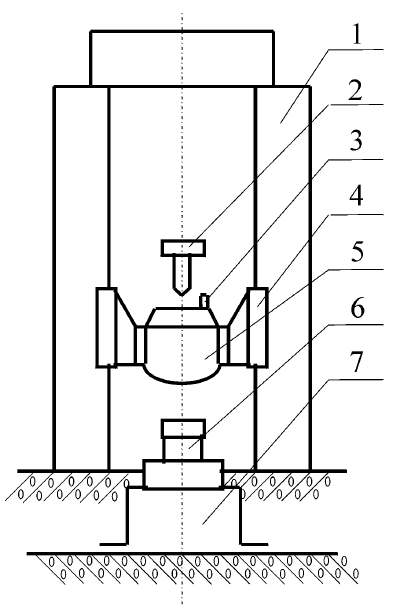
\includegraphics[width=0.3\textwidth]{example/cn_100t.png}\
  \begin{center}
    \small\kaishu 1.立柱 2.提升释放机构 3.标准冲击加速度计 \\ 4.导轨 5.重锤 6.被校力传感器 7.底座
  \end{center}
  \vspace{-1em}
  \bicaption[出现在插图索引中]
    {示例图片来源于\parencite{he1999}}
    {Stay hungry, stay foolish.}
 \label{fig:cn_100t}
\end{figure}

\subsection{绘制流程图}

图\ref{fig:flow_chart}是一张流程图示意。使用tikz环境,搭配四种预定义节点(\verb+startstop+、\verb+process+、\verb+decision+和\verb+io+),可以容易地绘制出流程图。
\begin{figure}[!htp]
    \centering
    \resizebox{6cm}{!}{\begin{tikzpicture}[node distance=2cm]
    \node (pic) [startstop] {待测图片};
    \node (bg) [io, below of=pic] {读取背景};
    \node (pair) [process, below of=bg] {匹配特征点对};
    \node (threshold) [decision, below of=pair, yshift=-0.5cm] {多于阈值};
    \node (clear) [decision, right of=threshold, xshift=3cm] {清晰?};
    \node (capture) [process, right of=pair, xshift=3cm, yshift=0.5cm] {重采};
    \node (matrix_p) [process, below of=threshold, yshift=-0.8cm] {透视变换矩阵};
    \node (matrix_a) [process, right of=matrix_p, xshift=3cm] {仿射变换矩阵};
    \node (reg) [process, below of=matrix_p] {图像修正};
    \node (return) [startstop, below of=reg] {配准结果};
     
    %连接具体形状
    \draw [arrow](pic) -- (bg);
    \draw [arrow](bg) -- (pair);
    \draw [arrow](pair) -- (threshold);

    \draw [arrow](threshold) -- node[anchor=south] {否} (clear);

    \draw [arrow](clear) -- node[anchor=west] {否} (capture);
    \draw [arrow](capture) |- (pic);
    \draw [arrow](clear) -- node[anchor=west] {是} (matrix_a);
    \draw [arrow](matrix_a) |- (reg);

    \draw [arrow](threshold) -- node[anchor=east] {是} (matrix_p);
    \draw [arrow](matrix_p) -- (reg);
    \draw [arrow](reg) -- (return);
\end{tikzpicture}
}
    \bicaption{绘制流程图效果}{Flow chart}
    \label{fig:flow_chart}
\end{figure}

\clearpage

\section{表格}
\label{sec:tab}

这一节给出的是一些表格的例子,如表\ref{tab:firstone}所示。

\begin{table}[!hpb]
  \centering
  \bicaption[指向一个表格的表目录索引]
    {一个颇为标准的三线表格\footnotemark[1]}
    {A Table}
  \label{tab:firstone}
  \begin{tabular}{@{}llr@{}} \toprule
    \multicolumn{2}{c}{Item} \\ \cmidrule(r){1-2}
    Animal & Description & Price (\$)\\ \midrule
    Gnat & per gram & 13.65 \\
    & each & 0.01 \\
    Gnu & stuffed & 92.50 \\
    Emu & stuffed & 33.33 \\
    Armadillo & frozen & 8.99 \\ \bottomrule
  \end{tabular}
\end{table}
\footnotetext[1]{这个例子来自\href{http://www.ctan.org/tex-archive/macros/latex/contrib/booktabs/booktabs.pdf}{《Publication quality tables in LATEX》}(booktabs宏包的文档)。这也是一个在表格中使用脚注的例子,请留意与threeparttable实现的效果有何不同。}

下面一个是一个更复杂的表格,用threeparttable实现带有脚注的表格,如表\ref{tab:footnote}。

\begin{table}[!htpb]
  \bicaption[出现在表目录的标题]
    {一个带有脚注的表格的例子}
    {A Table with footnotes}
  \label{tab:footnote}
  \centering
  \begin{threeparttable}[b]
     \begin{tabular}{ccd{4}cccc}
      \toprule
      \multirow{2}{6mm}{total}&\multicolumn{2}{c}{20\tnote{1}} & \multicolumn{2}{c}{40} &  \multicolumn{2}{c}{60}\\
      \cmidrule(lr){2-3}\cmidrule(lr){4-5}\cmidrule(lr){6-7}
      &www & \multicolumn{1}{c}{k} & www & k & www & k \\ % 使用说明符 d 的列会自动进入数学模式,使用 \multicolumn 对文字表头做特殊处理
      \midrule
      &$\underset{(2.12)}{4.22}$ & 120.0140\tnote{2} & 333.15 & 0.0411 & 444.99 & 0.1387 \\
      &168.6123 & 10.86 & 255.37 & 0.0353 & 376.14 & 0.1058 \\
      &6.761    & 0.007 & 235.37 & 0.0267 & 348.66 & 0.1010 \\
      \bottomrule
    \end{tabular}
    \begin{tablenotes}
    \item [1] the first note.% or \item [a]
    \item [2] the second note.% or \item [b]
    \end{tablenotes}
  \end{threeparttable}
\end{table}

\section{参考文献管理}

 \LaTeX 具有将参考文献内容和表现形式分开管理的能力,涉及三个要素:参考文献数据库、参考文献引用格式、在正文中引用参考文献。
这样的流程需要多次编译:

\begin{enumerate}[noitemsep,topsep=0pt,parsep=0pt,partopsep=0pt]
	\item 用户将论文中需要引用的参考文献条目,录入纯文本数据库文件(bib文件)。
	\item 调用xelatex对论文模板做第一次编译,扫描文中引用的参考文献,生成参考文献入口文件(aux)文件。
	\item 调用bibtex,以参考文献格式和入口文件为输入,生成格式化以后的参考文献条目文件(bib)。
	\item 再次调用xelatex编译模板,将格式化以后的参考文献条目插入正文。
\end{enumerate}

参考文献数据库(thesis.bib)的条目,可以从Google Scholar搜索引擎\footnote{\url{https://scholar.google.com}}、CiteSeerX搜索引擎\footnote{\url{http://citeseerx.ist.psu.edu}}中查找,文献管理软件Papers\footnote{\url{http://papersapp.com}}、Mendeley\footnote{\url{http://www.mendeley.com}}、JabRef\footnote{\url{http://jabref.sourceforge.net}}也能够输出条目信息。

下面是在Google Scholar上搜索到的一条文献信息,格式是纯文本:

\begin{lstlisting}[caption={从Google Scholar找到的参考文献条目}, label=googlescholar, escapeinside="", numbers=none]
    @phdthesis{"白2008信用风险传染模型和信用衍生品的定价",
      title={"信用风险传染模型和信用衍生品的定价"},
      author={"白云芬"},
      year={2008},
      school={"上海交通大学"}
    }
\end{lstlisting}

推荐修改后在bib文件中的内容为:

\begin{lstlisting}[caption={修改后的参考文献条目}, label=itemok, escapeinside="", numbers=none]
  @phdthesis{bai2008,
    title={"信用风险传染模型和信用衍生品的定价"},
    author={"白云芬"},
    date={2008},
    address={"上海"},
    school={"上海交通大学"}
  }
\end{lstlisting}

按照教务处的要求,参考文献外观应符合国标GBT7714的要求\footnote{\url{http://www.cces.net.cn/guild/sites/tmxb/Files/19798_2.pdf}}。
在模板中,表现形式的控制逻辑通过biblatex-gb7714-2015包实现\footnote{\url{https://www.ctan.org/pkg/biblatex-gb7714-2015}},基于{Bib\LaTeX}管理文献。在目前的多数TeX发行版中,可能都没有默认包含biblatex-gb7714-2015,需要手动安装。

正文中引用参考文献时,用\verb+\cite{key1,key2,key3...}+可以产生“上标引用的参考文献”,
如\cite{Meta_CN,chen2007act,DPMG}。
使用\verb+\parencite{key1,key2,key3...}+则可以产生水平引用的参考文献,例如\parencite{JohnD,zhubajie,IEEE-1363}。
请看下面的例子,将会穿插使用水平的和上标的参考文献:关于书的\parencite{Meta_CN,JohnD,IEEE-1363},关于期刊的\cite{chen2007act,chen2007ewi},
会议论文\parencite{DPMG,kocher99,cnproceed},
硕士学位论文\parencite{zhubajie,metamori2004},博士学位论文\cite{shaheshang,FistSystem01,bai2008},标准文件\parencite{IEEE-1363},技术报告\cite{NPB2},电子文献\parencite{xiaoyu2001, CHRISTINE1998},用户手册\parencite{RManual}。

总结一些注意事项:
\begin{itemize}
\item 参考文献只有在正文中被引用了,才会在最后的参考文献列表中出现;
\item 参考文献“数据库文件”bib是纯文本文件,请使用UTF-8编码,不要使用GBK编码;
\item 参考文献条目中默认通过date域输入时间。兼容使用year域时会产生编译warning,可忽略。
\end{itemize}

\section{用listings插入源代码}

原先ctexbook文档类和listings宏包配合使用时,代码在换页时会出现莫名其妙的错误,后来经高人指点,顺利解决了。
感兴趣的话,可以看看\href{http://bbs.ctex.org/viewthread.php?tid=53451}{这里}。
这里给使用listings宏包插入源代码的例子,这里是一段C代码。
另外,listings宏包真可谓博大精深,可以实现各种复杂、漂亮的效果,想要进一步学习的同学,可以参考
\href{http://mirror.ctan.org/macros/latex/contrib/listings/listings.pdf}{listings宏包手册}。

\begin{lstlisting}[language={C}, caption={一段C源代码}]
#include <stdio.h>
#include <unistd.h>
#include <sys/types.h>
#include <sys/wait.h>

int main() {
  pid_t pid;

  switch ((pid = fork())) {
  case -1:
    printf("fork failed\n");
    break;
  case 0:
    /* child calls exec */
    execl("/bin/ls", "ls", "-l", (char*)0);
    printf("execl failed\n");
    break;
  default:
    /* parent uses wait to suspend execution until child finishes */
    wait((int*)0);
    printf("is completed\n");
    break;
  }

  return 0;
}
\end{lstlisting}

\section{用algorithm和algorithmicx宏包插入算法描述}

algorithmicx 比 algorithmic 增加了一些命令。
示例如算法\ref{algo:sum_100}和算法\ref{algo:merge_sort},
后者的代码来自\href{http://hustsxh.is-programmer.com/posts/38801.html}{xhSong的博客}。
algorithmicx的详细使用方法见\href{http://mirror.hust.edu.cn/CTAN/macros/latex/contrib/algorithmicx/algorithmicx.pdf}{官方README}。
使用算法宏包时,算法出现的位置很多时候不按照tex文件里的书写顺序,
需要强制定位时可以使用\verb+\begin{algorithm}[H]+
\footnote{http://tex.stackexchange.com/questions/165021/fixing-the-location-of-the-appearance-in-algorithmicx-environment}

这是写在算法\ref{algo:sum_100}前面的一段话,在生成的文件里它会出现在算法\ref{algo:sum_100}前面。

\begin{algorithm}
% \begin{algorithm}[H] % 强制定位
\caption{求100以内的整数和}
\label{algo:sum_100}
\begin{algorithmic}[1] %每行显示行号
\Ensure 100以内的整数和 % 输出
\State $sum \gets 0$
\For{$i = 0 \to 100$}
    \State $sum \gets sum + i$
  \EndFor
\end{algorithmic}
\end{algorithm}

这是写在两个算法中间的一段话,当算法\ref{algo:sum_100}不使用\verb+\begin{algorithm}[H]+时它也会出现在算法\ref{algo:sum_100}前面。

对于很长的算法,单一的算法块\verb+\begin{algorithm}...\end{algorithm}+是不能自动跨页的
\footnote{http://tex.stackexchange.com/questions/70733/latex-algorithm-not-display-under-correct-section},
会出现的情况有:

\begin{itemize}
  \item 该页放不下当前的算法,留下大片空白,算法在下一页显示
  \item 单一页面放不下当前的算法,显示时超过页码的位置直到超出整个页面范围
\end{itemize}

解决方法有:

\begin{itemize}
  \item (推荐)使用\verb+algstore{algname}+和\verb+algrestore{algname}+来讲算法分为两个部分\footnote{http://tex.stackexchange.com/questions/29816/algorithm-over-2-pages},如算法\ref{algo:merge_sort}。
  \item 人工拆分算法为多个小的部分。
\end{itemize}

\begin{algorithm}
% \begin{algorithm}[H] % 强制定位
\caption{用归并排序求逆序数}
\label{algo:merge_sort}
\begin{algorithmic}[1] %每行显示行号
\Require $Array$数组,$n$数组大小 % 输入
\Ensure 逆序数 % 输出
\Function {MergerSort}{$Array, left, right$}
  \State $result \gets 0$
  \If {$left < right$}
    \State $middle \gets (left + right) / 2$
    \State $result \gets result +$ \Call{MergerSort}{$Array, left, middle$}
    \State $result \gets result +$ \Call{MergerSort}{$Array, middle, right$}
    \State $result \gets result +$ \Call{Merger}{$Array,left,middle,right$}
  \EndIf
  \State \Return{$result$}
\EndFunction
\State %空一行
\Function{Merger}{$Array, left, middle, right$}
  \State $i\gets left$
  \State $j\gets middle$
  \State $k\gets 0$
  \State $result \gets 0$
  \While{$i<middle$ \textbf{and} $j<right$}
    \If{$Array[i]<Array[j]$}
      \State $B[k++]\gets Array[i++]$
    \Else
      \State $B[k++] \gets Array[j++]$
      \State $result \gets result + (middle - i)$
    \EndIf
  \EndWhile
  \algstore{MergeSort}
\end{algorithmic}
\end{algorithm}

\begin{algorithm}
\begin{algorithmic}[1]
  \algrestore{MergeSort}
  \While{$i<middle$}
    \State $B[k++] \gets Array[i++]$
  \EndWhile
  \While{$j<right$}
    \State $B[k++] \gets Array[j++]$
  \EndWhile
  \For{$i = 0 \to k-1$}
    \State $Array[left + i] \gets B[i]$
  \EndFor
  \State \Return{$result$}
\EndFunction
\end{algorithmic}
\end{algorithm}

这是写在算法\ref{algo:merge_sort}后面的一段话,
但是当算法\ref{algo:merge_sort}不使用\verb+\begin{algorithm}[H]+时它会出现在算法\ref{algo:merge_sort}
甚至算法\ref{algo:sum_100}前面。

对于算法的索引要注意\verb+\caption+和\verb+\label+的位置,
必须是先\verb+\caption+再\verb+\label+\footnote{http://tex.stackexchange.com/questions/65993/algorithm-numbering},
否则会出现\verb+\ref{algo:sum_100}+生成的编号跟对应算法上显示不一致的问题。

根据Werner的回答\footnote{http://tex.stackexchange.com/questions/53357/switch-cases-in-algorithmic}
增加了\verb+Switch+和\verb+Case+的支持,见算法\ref{algo:switch_example}。

\begin{algorithm}
\caption{Switch示例}
\label{algo:switch_example}
\begin{algorithmic}[1]
  \Switch{$s$}
    \Case{$a$}
      \Assert{0}
    \EndCase
    \Case{$b$}
      \Assert{1}
    \EndCase
    \Default
      \Assert{2}
    \EndDefault
  \EndSwitch
\end{algorithmic}
\end{algorithm}

% %# -*- coding: utf-8-unix -*-
% !TEX program = xelatex
% !TEX root = ../thesis.tex
% !TEX encoding = UTF-8 Unicode
\chapter{常见问题}
\label{chap:faq}

{\bfseries{}Q:我是否能够自由使用这份模板?}

A:这份模板以Apache License 2.0开源许可证发布,请遵循许可证规范。

{\bfseries{}Q:我的论文是Word排版的,学校图书馆是不是只收 \LaTeX 排版的论文?}

A:当然不是,Word版论文肯定收。

{\bfseries{}Q:我的论文是 \LaTeX 排版的,学校图书馆是不是只收Word排版的论文?}

A:当然不是,PDF版的电子论文是可以上交的。是否要交Word版就看你导师的喜好了。

{\bfseries{}Q:为什么屏幕上显示的左右页边距不一样?}

A:模板默认是双面打印,迎面页和背面页的页边距是要交换的,多出来的那一部分是留作装订的。

{\bfseries{}Q:为什么在参考文献中会有“//”符号?}

A:那就是国标GBT7714参考文献风格规定的。但可以使用 gbpunctin=false 选项将其还原成 in:,进一步可以在导言区加入\verb+\DefineBibliographyStrings{english}{in={}}+将其去掉。

{\bfseries{}Q:为什么参考文献中会有[s.n.],[S.l], [EB/OL]等符号?}

A: 那也是国标GBT7714参考文献风格定义的。[s.n.]表示出版者不祥,[S.l]表示出版地不祥,[EB/OL]表示引用的参考文献类型为在线电子文档。但可以使用gbpub=false 选项将其缺省补充的出版项[s.n.]等去掉。也可以使用选项 gbtype=false 将参考文献类型标识去掉。

{\bfseries{}Q:如何获得帮助和反馈意见?}

A:你可以通过\href{https://github.com/sjtug/SJTUThesis/issues}{在github上开issue}
、在\href{https://bbs.sjtu.edu.cn/bbsdoc?board=TeX_LaTeX}{水源LaTeX版}发帖反映你使用过程中遇到的问题。

{\bfseries{}Q:使用文本编辑器查看tex文件时遇到乱码?}

A:请确保你的文本编辑器使用UTF-8编码打开了tex源文件。

{\bfseries{}Q:在CTeX编译模板遇到“rsfs10.tfm already exists”的错误提示?}

A:请删除\verb+X:\CTEX\UserData\fonts\tfm\public\rsfs+下的文件再重新编译。问题讨论见\href{https://bbs.sjtu.edu.cn/bbstcon,board,TeX_LaTeX,reid,1352982719.html}{水源2023号帖}。

{\bfseries{}Q:升级了TeXLive 2012,编译后的文档出现“minus”等字样?}

A:这是xltxtra和fontspec宏包导致的问题。学位论文模板从0.5起使用metatlog宏包代替xltxtra生成 \XeTeX 标志,解决了这个问题。

{\bfseries{}Q:为什么在bib中加入的参考文献,没有在参考文献列表中出现?}

A: bib中的参考文献条目,常通过\verb+\cite+或\verb+\parencite+或\verb+\supercite+或\verb+\textcite+等命令在正文中引用进而加入到参考文献列表中。当需要将参考文献条目加入到文献表中但又不引用可以使用\verb+\nocite+命令,当nocite参数为*时则引入bib中的所有文献。
%\verb+\upcite+ 是哪个宏包的?之前没有见过

{\bfseries{}Q:我可以使用Sublime Text编写学位论文吗?}

A: 可以。首先\href{https://www.sublimetext.com/}{下载}并安装Sublime Text,然后安装
\href{https://packagecontrol.io/installation}{Package Control},
之后按\verb|ctrl+shift+p|或者\verb|cmd+shift+p|调出命令窗口,
输入\verb|install|,选择\textit{Package Control: Install Package},按回车,
稍等片刻,等待索引载入后会弹出选项框,输入\verb|LaTeXTools|并回车,即可成功安装插件。
之后只需要打开\verb|.tex|文件,按\verb|ctrl+b|或者\verb|cmd+b|即可编译,
如有错误,双击错误信息可以跳转到出错的行。

{\bfseries{}Q:在macTex中,为什么pdf图片无法插入?}

A:如果报错是“pdf: image inclusion failed for "./figure/chap2/sjtulogo.pdf".”,则采取以下步骤

\begin{lstlisting}[basicstyle=\small\ttfamily, caption={编译模板}, numbers=none]
brew install xpdf
wget http://mirrors.ctan.org/support/epstopdf.zip
unzip epstopdf.zip
cp epstopdf/epstopdf.pl /usr/local/bin/
cd figure/chap2
pdftops sjtulogo.pdf
epstopdf sjtulogo.ps
pdfcrop sjtulogo.pdf
mv sjtulogo.pdf backup.pdf
mv sjtulogo-crop.pdf sjtulogo.pdf
\end{lstlisting}

{\bfseries{}Q:为什么维普等查重系统无法识别此模板生成的 pdf 内所有的中文?}

A: 中文无法识别的情况多半是由于使用了 ShareLaTeX 的原因,请尝试使用 TexStudio 等软件在本地进行编译。
如果使用 TeXstudio 请在 Preferences-Build 中将 Default Compiler 和 Default Bibliography Tool 分别改为 XeLaTeX 和 Biber。

{\bfseries{}Q:如何向你致谢?}

A: 烦请在模板的\href{https://github.com/sjtug/SJTUThesis}{github主页}点击“Star”,我想粗略统计一下使用学位论文模板的人数,谢谢大家。非常欢迎大家向项目贡献代码。

% %# -*- coding: utf-8-unix -*-
% !TEX program = xelatex
% !TEX root = ../thesis.tex
% !TEX encoding = UTF-8 Unicode
%%==================================================
%% conclusion.tex for SJTUThesis
%% Encoding: UTF-8
%%==================================================

\begin{summary}

这里是全文总结内容。

2015年2月28日,中央在北京召开全国精神文明建设工作表彰暨学雷锋志愿服务大会,公布全国文明城市(区)、文明村镇、文明单位名单。上海交通大学荣获全国文明单位称号。         

全国文明单位这一荣誉是对交大人始终高度重视文明文化工作的肯定,是对交大长期以来文明创建工作成绩的褒奖。在学校党委、文明委的领导下,交大坚持将文明创建工作纳入学校建设世界一流大学的工作中,全体师生医护员工群策群力、积极开拓,落实国家和上海市有关文明创建的各项要求,以改革创新、科学发展为主线,以质量提升为目标,聚焦文明创建工作出现的重点和难点,优化文明创建工作机制,传播学校良好形象,提升社会美誉度,显著增强学校软实力。2007至2012年间,上海交大连续三届荣获“上海市文明单位”称号,成为创建全国文明单位的新起点。         

上海交大自启动争创全国文明单位工作以来,凝魂聚气、改革创新,积极培育和践行社会主义核心价值观。坚持统筹兼顾、多措并举,将争创全国文明单位与学校各项中心工作紧密结合,着力构建学校文明创建新格局,不断提升师生医护员工文明素养,以“冲击世界一流大学汇聚强大精神动力”为指导思想,以“聚焦改革、多元推进、以评促建、丰富内涵、彰显特色”为工作原则,并由全体校领导群策领衔“党的建设深化、思想教育深入、办学成绩显著、大学文化丰富、校园环境优化、社会责任担当”六大板块共28项重点突破工作,全面展现近年来交大文明创建工作的全貌和成就。         

进入新阶段,学校将继续开拓文明创建工作新格局,不断深化工作理念和工作实践,创新工作载体、丰富活动内涵、凸显创建成效,积极服务于学校各项中心工作和改革发展的大局面,在上级党委、文明委的关心下,在学校党委的直接领导下,与时俱进、开拓创新,为深化内涵建设、加快建成世界一流大学、推动国家进步和社会发展而努力奋斗!       

上海交通大学医学院附属仁济医院也获得全国文明单位称号。      

\end{summary}


\appendix % 使用英文字母对附录编号

% 附录内容,本科学位论文可以用翻译的文献替代。
% %# -*- coding: utf-8-unix -*-
% !TEX program = xelatex
% !TEX root = ../thesis.tex
% !TEX encoding = UTF-8 Unicode
\chapter{搭建模板编译环境}

\section{安装TeX发行版}

\subsection{Mac OS X}

Mac用户可以从MacTeX主页\footnote{\url{https://tug.org/mactex/}}下载MacTeX。
也可以通过brew包管理器\footnote{\url{http://caskroom.io}}安装MacTeX。

\begin{lstlisting}[basicstyle=\small\ttfamily, numbers=none]
brew cask install mactex
\end{lstlisting}

\subsection{Linux}

建议Linux用户使用TeXLive主页\footnote{\url{https://www.tug.org/texlive/}}的脚本来安装TeXLive。
以下命令将把TeXLive发行版安装到当前用户的家目录下。
若计划安装一个供系统上所有用户使用的TeXLive,请使用root账户操作。

\begin{lstlisting}[basicstyle=\small\ttfamily, numbers=none]
wget http://mirror.ctan.org/systems/texlive/tlnet/install-tl-unx.tar.gz
tar xzvpf install-tl-unx.tar.gz
cd install-tl-20150411/
./install-tl
\end{lstlisting}

\section{安装中文字体}

\subsection{Mac OS X、Deepin}

Mac和Deepin用户双击字体文件即可安装字体。

\subsection{RedHat/CentOS用户}

RedHat/CentOS用户请先将字体文件复制到字体目录下,调用fc-cache刷新缓存后即可在TeXLive中使用新字体。

\begin{lstlisting}[basicstyle=\small\ttfamily, numbers=none]
mkdir ~/.fonts
cp *.ttf ~/.fonts				# 当前用户可用新字体
cp *.ttf /usr/share/fonts/local/	# 所有用户可以使用新字体
fc-cache -f
\end{lstlisting}


% %# -*- coding: utf-8-unix -*-
% !TEX program = xelatex
% !TEX root = ../thesis.tex
% !TEX encoding = UTF-8 Unicode
%% app2.tex for SJTU Master Thesis
%% based on CASthesis
%% modified by wei.jianwen@gmail.com
%% version: 0.3a
%% Encoding: UTF-8
%% last update: Dec 5th, 2010
%%==================================================

\chapter{Maxwell Equations}

选择二维情况,有如下的偏振矢量:
\begin{subequations}
  \begin{eqnarray}
    {\bf E}&=&E_z(r,\theta)\hat{\bf z} \\
    {\bf H}&=&H_r(r,\theta))\hat{ \bf r}+H_\theta(r,\theta)\hat{\bm
      \theta}
  \end{eqnarray}
\end{subequations}
对上式求旋度:
\begin{subequations}
  \begin{eqnarray}
    \nabla\times{\bf E}&=&\frac{1}{r}\frac{\partial E_z}{\partial\theta}{\hat{\bf r}}-\frac{\partial E_z}{\partial r}{\hat{\bm\theta}}\\
    \nabla\times{\bf H}&=&\left[\frac{1}{r}\frac{\partial}{\partial
        r}(rH_\theta)-\frac{1}{r}\frac{\partial
        H_r}{\partial\theta}\right]{\hat{\bf z}}
  \end{eqnarray}
\end{subequations}
因为在柱坐标系下,$\overline{\overline\mu}$是对角的,所以Maxwell方程组中电场$\bf E$的旋度:
\begin{subequations}
  \begin{eqnarray}
    &&\nabla\times{\bf E}=\mathbf{i}\omega{\bf B} \\
    &&\frac{1}{r}\frac{\partial E_z}{\partial\theta}{\hat{\bf
        r}}-\frac{\partial E_z}{\partial
      r}{\hat{\bm\theta}}=\mathbf{i}\omega\mu_rH_r{\hat{\bf r}}+\mathbf{i}\omega\mu_\theta
    H_\theta{\hat{\bm\theta}}
  \end{eqnarray}
\end{subequations}
所以$\bf H$的各个分量可以写为:
\begin{subequations}
  \begin{eqnarray}
    H_r=\frac{1}{\mathbf{i}\omega\mu_r}\frac{1}{r}\frac{\partial
      E_z}{\partial\theta } \\
    H_\theta=-\frac{1}{\mathbf{i}\omega\mu_\theta}\frac{\partial E_z}{\partial r}
  \end{eqnarray}
\end{subequations}
同样地,在柱坐标系下,$\overline{\overline\epsilon}$是对角的,所以Maxwell方程组中磁场$\bf H$的旋度:
\begin{subequations}
  \begin{eqnarray}
    &&\nabla\times{\bf H}=-\mathbf{i}\omega{\bf D}\\
    &&\left[\frac{1}{r}\frac{\partial}{\partial
        r}(rH_\theta)-\frac{1}{r}\frac{\partial
        H_r}{\partial\theta}\right]{\hat{\bf
        z}}=-\mathbf{i}\omega{\overline{\overline\epsilon}}{\bf
      E}=-\mathbf{i}\omega\epsilon_zE_z{\hat{\bf z}} \\
    &&\frac{1}{r}\frac{\partial}{\partial
      r}(rH_\theta)-\frac{1}{r}\frac{\partial
      H_r}{\partial\theta}=-\mathbf{i}\omega\epsilon_zE_z
  \end{eqnarray}
\end{subequations}
由此我们可以得到关于$E_z$的波函数方程:
\begin{eqnarray}
  \frac{1}{\mu_\theta\epsilon_z}\frac{1}{r}\frac{\partial}{\partial r}
  \left(r\frac{\partial E_z}{\partial r}\right)+
  \frac{1}{\mu_r\epsilon_z}\frac{1}{r^2}\frac{\partial^2E_z}{\partial\theta^2}
  +\omega^2 E_z=0
\end{eqnarray}

% %# -*- coding: utf-8-unix -*-
% !TEX program = xelatex
% !TEX root = ../thesis.tex
% !TEX encoding = UTF-8 Unicode
\chapter{从 {\CJKLaTeX} 转向 \texorpdfstring{\XeTeX}{XeTeX}}
\label{chap:whydvipdfm}

我习惯把v0.2a使用dvipdfmx编译的硕士学位论文模板称为“ \CJKLaTeX 模板”,而这个使用 \XeTeX 引擎(xelatex程序)处理的模板则被称为“{\XeTeX/\LaTeX}模板”。
从 \CJKLaTeX 模板迁移到{\XeTeX\LaTeX}模板的好处有下:
\begin{enumerate}
\item[\large\smiley] 搭建 \XeTeX 环境比搭建 \CJKLaTeX 环境更容易;
\item[\large\smiley] 更简单的字体控制;
\item[\large\smiley] 完美支持PDF/EPS/PNG/JPG图片,不需要“bound box(.bb)”文件;
\item[\large\smiley] 支持OpenType字体的复杂字型变化功能;
\end{enumerate}

当然,这也是有代价的。由于 \XeTeX 比较新,在我看来,使用 \XeTeX 模板所必须付出的代价是:

\begin{enumerate}
\item[\large\frownie] 必须把你“古老的” \TeX 系统更新为较新的版本。TeXLive 2012和CTeX 2.9.2能够编译这份模板,而更早的版本则无能为力。
\item[\large\frownie] 需要花一些时间把你在老模板上的工作迁移到新模板上。
\end{enumerate}

第一条就看你如何取舍了,新系统通常意味着更好的兼容性,值得升级。而转换模板也不是什么特别困难的事情,可以这样完成:

\begin{enumerate}
\item 备份你要转换的源文件,以防你的工作成果丢失;
\item 将你原来的tex以及bib文件另存为UTF-8编码的文件。iconv、vim、emacs、UEdit等等工具都可以完成。WinEdt对文件编码识别功能很差(到了v6.0还是如此),不推荐作为字符编码转换工具;
\item 将diss.tex导言区中的内容替换为XeTeX模板diss.tex导言区的内容;
\item 将你对原先导言区的修改,小心翼翼地合并到新的导言区中;
\item 使用XeTeX模板中的GBT7714-2005NLang.bst替换原有的bst文件,新的bst文件只是将字符编码转换为UTF-8;
\item 删除bouding box文件;
\item 使用本文\ref{sec:process}介绍的方法,重新编译文档;
\end{enumerate}


% %# -*- coding: utf-8-unix -*-
% !TEX program = xelatex
% !TEX root = ../thesis.tex
% !TEX encoding = UTF-8 Unicode
\chapter{模板更新记录}
\label{chap:updatelog}

\textbf{2018年1月} v0.10发布,项目转移至 \href{https://github.com/sjtug/SJTUThesis}{SJTUG} 名下,并增加了英文模版,修改了默认字体设置。

\textbf{2016年12月} v0.9.5发布,改用GB7714-2015参考文献风格。

\textbf{2016年11月} v0.9.4发布,增加算法和流程图。

\textbf{2015年6月19日} v0.9发布,适配ctex 2.x宏包,需要使用TeXLive 2015编译。

\textbf{2015年3月15日} v0.8发布,使用biber/biblatex组合替代 \BibTeX ,带来更强大稳定的参考文献处理能力;添加enumitem宏包增强列表环境控制能力;完善宏包文字描述。

\textbf{2015年2月15日} v0.7发布,增加盲审选项,调用外部工具插入扫描件。

\textbf{2015年2月14日} v0.6.5发布,修正一些小问题,缩减git仓库体积,仓库由sjtu-thesis-template-latex更名为SJTUThesis。

\textbf{2014年12月17日} v0.6发布,学士、硕士、博士学位论文模板合并在了一起。

\textbf{2013年5月26日} v0.5.3发布,更正subsubsection格式错误,这个错误导致如"1.1 小结"这样的标题没有被正确加粗。

\textbf{2012年12月27日} v0.5.2发布,更正拼写错误。在diss.tex加入ack.tex。

\textbf{2012年12月21日} v0.5.1发布,在 \LaTeX 命令和中文字符之间留了空格,在Makefile中增加release功能。

\textbf{2012年12月5日} v0.5发布,修改说明文件的措辞,更正Makefile文件,使用metalog宏包替换xltxtra宏包,使用mathtools宏包替换amsmath宏包,移除了所有CJKtilde(\verb+~+)符号。

\textbf{2012年5月30日} v0.4发布,包含交大学士、硕士、博士学位论文模板。模板在\href{https://github.com/sjtug/SJTUThesis}{github}上管理和更新。

\textbf{2010年12月5日} v0.3a发布,移植到 \XeTeX/\LaTeX 上。

\textbf{2009年12月25日} v0.2a发布,模板由CASthesis改名为sjtumaster。在diss.tex中可以方便地改变正文字号、切换但双面打印。增加了不编号的一章“全文总结”。
添加了可伸缩符号(等号、箭头)的例子,增加了长标题换行的例子。

\textbf{2009年11月20日} v0.1c发布,增加了Linux下使用ctex宏包的注意事项、.bib条目的规范要求,
修正了ctexbook与listings共同使用时的断页错误。

\textbf{2009年11月13日} v0.1b发布,完善了模板使用说明,增加了定理环境、并列子图、三线表格的例子。

\textbf{2009年11月12日} 上海交通大学硕士学位论文 \LaTeX 模板发布,版本0.1a。



\backmatter % 文后无编号部分

% 参考资料
\printbibliography[heading=bibintoc]

% 致谢、发表论文、申请专利、参与项目、简历
% 用于盲审的论文需隐去致谢、发表论文、申请专利、参与的项目
\makeatletter

\ifsjtu@coursepaper
\else

  % "研究生学位论文送盲审印刷格式的统一要求"
  % http://www.gs.sjtu.edu.cn/inform/3/2015/20151120_123928_738.htm

  % 盲审删去删去致谢页
  \ifsjtu@review\relax\else
    %# -*- coding: utf-8-unix -*-
% !TEX program = xelatex
% !TEX root = ../thesis.tex
% !TEX encoding = UTF-8 Unicode
%TC:ignore
\begin{thanks}

感谢我的毕业设计指导老师王肇国副教授在本项目中对我给予的指导与帮助。

感谢上海交通大学软件学院的老师们对我的在专业技能上的培养。

感谢亲爱的同学与朋友们在本科四年期间对我给予支持,与我分享欢乐,我将永远珍惜这段难忘的时光。

感谢我的父母,来自他们的鼓励是我最困难时的支撑,与他们的讨论是我最迷茫时的明灯,他们是世界上最棒的父母。

\end{thanks}
%TC:endignore
         % 致谢
  \fi

  \ifsjtu@bachelor
    % 学士学位论文要求在最后有一个英文大摘要,单独编页码
    %# -*- coding: utf-8-unix -*-
% !TEX program = xelatex
% !TEX root = ../thesis.tex
% !TEX encoding = UTF-8 Unicode
\begin{bigabstract}
The recent proposal of learned index structures opens up a new perspective on how traditional range indexes can be optimized.
The pioneer study on learned index structures arouses a lot of excitements around how machine learning can resculpt system components that have been decades-old, such as bloom filters, join queries or even enable self-tuning databases.

The insight is that indexes can be viewed as functions from the data (key) to the values representing either record positions in a sorted array (for range index), in an unsorted array (for Hash-Index) or whether the data exists or not (for BitMap-Index).
For the case of range index, the function is effectively a cumulative distribution function (CDF).
Given the CDF $F$, the positions can be predicted by: $p=F(\text{Key})*N$ where $p$ is the position of the key and $N$ is the total number of keys.

The core idea is to approximate the CDF function $F$ by machine learning models such as deep neural networks.
While the choice of the model architectures can vary, the paper proposes a \emph{staged model} architecture inspired by the multi-stage structure of B-Tree.
The sub-model at each stage predicts which sub-models to be activated in the next stage while the leaf stage directly predicts the CDF values.
The model is trained from the root stage to the leaf stage, and each stage is trained separately using the following loss function: $L_l=\sum_{(x,y)}(f_l^{(\lfloor M_lf_{l-1}(x)/N\rfloor )}(x)-y)^2~;~L_0=\sum_{(x,y)}(f_0(x)-y)^2$.
Here, $(x,y)$ is the key/position pair from the data to be indexed; $L_l$ is the loss function of stage $l$; $f_l^{(k)}$ is the $k^{th}$ sub-model of stage $l$.
$f_{l-1}$ recursively executes the above equation until the root stage $L_0$.

To deploy the learned index, the approximation error needs to be corrected.
First, the prediction error can be bounded by looking at the maximum distance $\sigma$ between the predicted and the true positions for each key.
Hence, if $pos$ is the predicted position by the learned index, the true position is guaranteed to be within $[pos-\sigma, pos+\sigma]$, and a binary search can be used.
The error bound $\sigma$ is thus a critical indicator of the effectiveness of the learned index.
The smaller $\sigma$ is, the more effective is the index.

However, the current learned indexes assume the data distribution is relatively static and the access pattern is uniform, while real-world scenarios consist of skew query distribution and evolving data.
These two issues hinder the wider adoption of the learned indexes for real-world workloads.
In this paper, we demonstrate that the missing consideration of access patterns and dynamic data distribution notably hinders the applicability of learned indexes.

Their preliminary study assumes a relatively static distribution function, while in many real world scenarios, the data is constantly evolving.
Typical approaches simply rely on re-training the whole model once the data distribution shifts notably from the training set used by the current model.
However, such re-training is costly, because not only the model parameters need to be \textit{fine-tuned}, but also that the model architecture needs to be searched again for better accuracy.
An advantage of using complex models (e.g., neural networks) at the first stage is that it can approximate the complex distribution which cannot be fitted with linear model.
As a result, for those distributions, the complex network is able to dispatch the data more evenly than simple models, which is good for the uniform workload.
However, \textbf{complex model is good for the complex distribution, but not always.}
This is because of the computation cost of complex models.
With the first stage model getting more complex, even though the binary search time decreases, but the model computation time increases.
Because of this tradeoff, though for some distributions that complex models like neural networks can save the binary search time, using linear model can achieve better the overall query time.
As a result, no heuristics can precisely tell which model architecture should be used.
Depending on the size of the hyperparamter search space, a basic architecture search technique such as grid search can easily take up to 10-100x the model training time.

Besides the inefficiency in handling dynamic workloads, the learned index paper also assumes a uniform access pattern (or query distribution).
However, queries in real worlds tend to be skew, where some keys are much more frequently queried than the others.
Querying a key with learned index has two steps: first, it predicts the position by model computation; Second, it tries to find the actual position using binary search in a bounded range.
However, its latency usually depends on the binary search, as it takes much longer time than model computation, in our evaluation.
Further, the search area is decided by the error bound\footnote{the difference between minimum and maximum prediction error} of the last stage model who has the key.
Thus, we have the following observation.
\textbf{A skew workload's performance is dominated by the hot models' error bound.}
Hot model is defined as the last stage model who holds a hot (frequently accessed) key.
Given a workload, all models' error bounds can vary across different model architectures, including the hot models'.
As a result, predicting a hot key with large model error bound is way more expensive, and we show that the originally proposed learned index model performs poorly under such scenarios.

In this paper, we propose \sys, a new learned index system for dynamic workloads where the data distribution and access pattern may be skew and evolving.
\sys incorporates read access pattern using the \textbf{Training Set Generator} and the \textbf{Finalizer} and reuses pre-trained models using the \textbf{Counselor}.
To handle skewed access pattern, we first investigate and discuss why the original model fails to address this issue.
To improve the latency for skew queries, \sys augments the training data with access frequencies.
For the issue of model re-training, our insight is that the same model architecture can be reused for similar data distribution and access pattern.
To address the slow model re-training when data distribution shifts, \sys caches the previously-trained models and incrementally fine-tunes them for similar access patterns and data distribution.

Training Set Generator takes the workload and dataset as input, extracts the access pattern by uniformly sampling from the workload and ``stretches'' the dataset according to the access pattern.
Then it sends the stretched training set to Counselor to get a tuned model.
Instead of improving the prediction accuracy of the hot keys, \sys focus on the error bounds of the models containing the hot keys (hot models).
Since the models assigned with few keys tend to have small error bounds, we try to reduce the number of keys handled by the hot models by ``stretching'' the dataset.
If a key is frequently accessed, we would like to increase the distance between it with its neighbors, the key before or after it.
It can be achieved by simply multiplying the position labels be the cumulative access frequency of given keys.
% Specifically, given a key with position $p$ before ``stretching'', if its access frequency is $f$, and the dataset size is $N$ then we need to shift its position to be $p + (n-1)/2$, and shift all keys after it with $n-1$.
% For the above example, the training set of \{(a, 0), (b, 1), (c, 2)\} with access frequency 1:2:1 will be augmented to be \{(a, 0), (b, 1.5), (c, 3)\}.
% Figure~\ref{fig:stretch} shows the CDF of dataset 1 before and after ``stretching'' with the access pattern in workload Skewed 3.

After incorporating the access pattern, the only factor affecting the model architecture is data distribution.
We notice that the best model architecture tends to be the same for similar data distributions.
As a result, \sys is able to cache a mapping from data distributions to models for future reusing.
This is done by the Counselor component, which includes four modules: Analyzer, Model Cache, Fine Tuner and Auto-tuner.
Analyzer extracts distribution information by uniformly sampling $K$ records from the generated training set, then normalize both key and position to [0, 1].
However, $K$ needs to be large enough to avoid breaking the distribution.
Model Cache maintains a mapping from the distribution of previous training set to their learning model's architure and parameters.
If it receives a distribution from Analyzer, it will finds the entry in the map with the most similar distribution based on the mean square error.
Then, it will send the model's information in that entry to Fine Tuner.
Furthermore, if the similarity is below a threshold, it will also start the auto-tuning process.
Fine Tuner incrementally trains the model retrieved from the model cache with the training set.
Auto-tuner uses grid search to find the best model architecture in the given search space.
It performs auto-tuning at the background and sends the result to the Finalizer component.

Before using the returned model from Counselor, the Finalizer needs to retrain the last stage models with the original dataset.
This is because the position of each key in the stretched training set is changed, we need to repair the position information with the original dataset.
This process is considerably fast as last models are usually linear models.
% For example, it only takes 118 $\mu$s to retrain one last model with 1000 keys.

The preliminary result shows that, by augmenting dataset with the access frequency, the best model architecture has 45.1\% performance improvement; by caching and reusing previous training result, the rebuilding time is reduced to XXX.

\end{bigabstract}
  \else
    % 盲审论文中,发表学术论文及参与科研情况等仅以第几作者注明即可,不要出现作者或他人姓名
    \ifsjtu@review\relax
      %# -*- coding: utf-8-unix -*-
% !TEX program = xelatex
% !TEX root = ../thesis.tex
% !TEX encoding = UTF-8 Unicode
%TC:ignore
\begin{publications}{99}
    \item\textsc{第一作者}. {中文核心期刊论文}, 2007.
    \item\textsc{第一作者}. {EI国际会议论文}, 2006.
\end{publications}
%TC:endignore

      %# -*- coding: utf-8-unix -*-
% !TEX program = xelatex
% !TEX root = ../thesis.tex
% !TEX encoding = UTF-8 Unicode
%TC:ignore
\begin{projects}{99}
    \item 参与973项目子课题(2007年6月--2008年5月)
    \item 参与自然基金项目(2005年5月--2005年8月)
    \item 参与国防项目(2005年8月--2005年10月)
\end{projects}
%TC:endignore

    \else
      %# -*- coding: utf-8-unix -*-
% !TEX program = xelatex
% !TEX root = ../thesis.tex
% !TEX encoding = UTF-8 Unicode
%%==================================================
%% pub.tex for SJTUThesis
%% Encoding: UTF-8
%%==================================================
%TC:ignore
\begin{publications}{99}
    \item\textsc{Chen H, Chan C~T}. {Acoustic cloaking in three dimensions using acoustic metamaterials}[J]. Applied Physics Letters, 2007, 91:183518.
    \item\textsc{Chen H, Wu B~I, Zhang B}, et al. {Electromagnetic Wave Interactions with a Metamaterial Cloak}[J]. Physical Review Letters, 2007, 99(6):63903.
\end{publications}
%TC:endignore
       % 发表论文
      %# -*- coding: utf-8-unix -*-
% !TEX program = xelatex
% !TEX root = ../thesis.tex
% !TEX encoding = UTF-8 Unicode
%%==================================================
%% projects.tex for SJTUThesis
%% Encoding: UTF-8
%%==================================================
%TC:ignore
\begin{projects}{99}
    \item 973项目“XXX”
    \item 自然基金项目“XXX”
    \item 国防项目“XXX”
\end{projects}
%TC:endignore
  % 参与的项目
      % %# -*- coding: utf-8-unix -*-
% !TEX program = xelatex
% !TEX root = ../thesis.tex
% !TEX encoding = UTF-8 Unicode
%TC:ignore
\begin{patents}{99}
    \item 第一发明人,“永动机”,专利申请号202510149890.0
\end{patents}
%TC:endignore
   % 申请专利
      %TC:ignore
\begin{resume}
  \begin{resumesection}{基本情况}
    某某,yyyy 年 mm 月生于 xxxx。
  \end{resumesection}

  \begin{resumelist}{教育背景}
    \item yyyy 年 mm 月至今,上海交通大学,博士研究生,xx 专业
    \item yyyy 年 mm 月至 yyyy 年 mm 月,上海交通大学,硕士研究生,xx 专业
    \item yyyy 年 mm 月至 yyyy 年 mm 月,上海交通大学,本科,xx 专业
  \end{resumelist}

  \begin{resumesection}{研究兴趣}
    \LaTeX{} 排版
  \end{resumesection}

  \begin{resumelist}{联系方式}
    \item 地址: 上海市闵行区东川路 800 号,200240
    \item E-mail: \email{xxx@sjtu.edu.cn}
  \end{resumelist}
\end{resume}
%TC:endignore
    % 个人简历
    \fi
  \fi
\fi

\makeatother

\end{document}
